\documentclass[12pt]{article}\usepackage[]{graphicx}\usepackage[]{color}
% maxwidth is the original width if it is less than linewidth
% otherwise use linewidth (to make sure the graphics do not exceed the margin)
\makeatletter
\def\maxwidth{ %
  \ifdim\Gin@nat@width>\linewidth
    \linewidth
  \else
    \Gin@nat@width
  \fi
}
\makeatother

\definecolor{fgcolor}{rgb}{0.345, 0.345, 0.345}
\newcommand{\hlnum}[1]{\textcolor[rgb]{0.686,0.059,0.569}{#1}}%
\newcommand{\hlstr}[1]{\textcolor[rgb]{0.192,0.494,0.8}{#1}}%
\newcommand{\hlcom}[1]{\textcolor[rgb]{0.678,0.584,0.686}{\textit{#1}}}%
\newcommand{\hlopt}[1]{\textcolor[rgb]{0,0,0}{#1}}%
\newcommand{\hlstd}[1]{\textcolor[rgb]{0.345,0.345,0.345}{#1}}%
\newcommand{\hlkwa}[1]{\textcolor[rgb]{0.161,0.373,0.58}{\textbf{#1}}}%
\newcommand{\hlkwb}[1]{\textcolor[rgb]{0.69,0.353,0.396}{#1}}%
\newcommand{\hlkwc}[1]{\textcolor[rgb]{0.333,0.667,0.333}{#1}}%
\newcommand{\hlkwd}[1]{\textcolor[rgb]{0.737,0.353,0.396}{\textbf{#1}}}%
\let\hlipl\hlkwb

\usepackage{framed}
\makeatletter
\newenvironment{kframe}{%
 \def\at@end@of@kframe{}%
 \ifinner\ifhmode%
  \def\at@end@of@kframe{\end{minipage}}%
  \begin{minipage}{\columnwidth}%
 \fi\fi%
 \def\FrameCommand##1{\hskip\@totalleftmargin \hskip-\fboxsep
 \colorbox{shadecolor}{##1}\hskip-\fboxsep
     % There is no \\@totalrightmargin, so:
     \hskip-\linewidth \hskip-\@totalleftmargin \hskip\columnwidth}%
 \MakeFramed {\advance\hsize-\width
   \@totalleftmargin\z@ \linewidth\hsize
   \@setminipage}}%
 {\par\unskip\endMakeFramed%
 \at@end@of@kframe}
\makeatother

\definecolor{shadecolor}{rgb}{.97, .97, .97}
\definecolor{messagecolor}{rgb}{0, 0, 0}
\definecolor{warningcolor}{rgb}{1, 0, 1}
\definecolor{errorcolor}{rgb}{1, 0, 0}
\newenvironment{knitrout}{}{} % an empty environment to be redefined in TeX

\usepackage{alltt}
\usepackage[utf8]{inputenc}
\usepackage[german]{babel}
\usepackage{apacite}
\usepackage{graphicx}
\usepackage{amsmath}
\usepackage{xcolor}
\usepackage{a4wide}
\usepackage[nottoc, numbib]{tocbibind}
\usepackage{natbib} 
\usepackage{booktabs}
\usepackage{longtable}
\usepackage{array}
\usepackage{multirow}
\usepackage{wrapfig}
\usepackage{float}
\usepackage{colortbl}
\usepackage{pdflscape}
\usepackage{tabu}
\usepackage{threeparttable}
\usepackage{threeparttablex}
\usepackage[normalem]{ulem}
\usepackage{makecell}
\usepackage{siunitx}
\usepackage{caption}
\usepackage{setspace}
\captionsetup{font=footnotesize}




\title{Konzept der Multilevel Analyse und deren Vorteil\\ \large{Erkenntnisse einer Simulationsstudie in R}}

\author{Masterarbeit von \\ Noah Bosshart \\ Mat-Nr.: 13-747-141 \\ \\ \\ Betreut durch \\ Prof. Dr. Carolin Strobl}
\IfFileExists{upquote.sty}{\usepackage{upquote}}{}
\begin{document}
\setstretch{1.5}

\begin{figure}[t]
  \centering
  
\includegraphics[width = 8cm]{uzh_logo}
\end{figure}

\maketitle
\thispagestyle{empty}

\newpage
\pagenumbering{Roman}
\tableofcontents

\newpage
\listoffigures

\newpage
\listoftables
\newpage


\section{Abstract}
\newpage

\pagenumbering{arabic}
\section{Einleitung}
Hierarchische Daten treten häufig in den Sozialwissenschaften auf, unter anderem auch in der Psychologie \citep{SnijdersTomA.B2012Ma:a}. Von hierarchischen Daten wird gesprochen, wenn beispielsweise Daten von Schulkindern innerhalb verschiedener Schulklassen oder von Mitarbeitern aus mehreren Teams erhoben werden. Aber auch Daten aus Langzeitstudien werden als gruppiert bezeichnet, da mehrere Messzeitpunkte innerhalb einer Person gruppiert sind. Hierarchische Daten werden in Levels unterteilt, wobei Daten aus der niedrigsten Stufe als Level-1 Einheiten bezeichnet werden \citep{SnijdersTomA.B2012Ma:a}. Ein Beispiel für Level-1 Einheiten sind Schulkinder. Diese Schulkinder befinden sich wiederum in Klassen, die in der Hierarchiestufe höher sind und folglich als Level-2 Einheiten bezeichnet werden. Würde man nun in einer Studie nicht nur Schulkinder in Schulklassen, sondern auch  die Schulen selbst berücksichtigen, würden die Schulen als Level-3 Einheit bezeichnet werden. Die Anzahl der Levels könnte man theoretisch beliebig hoch wählen, solange es das Studiendesign erlaubt und es aus der Perspektive der Forschungsfrage sinnvoll ist. Der Einfachheit halber beschränken wir uns im Laufe dieser Arbeit aber auf hierarchische Daten mit zwei Levels. In Tabelle \ref{tab:beispiele_levels} werden einige Beispiele für Level-1 und Level-2 Einheiten aufgeführt. 
\begin{table}[h!]
\centering
\caption{Beispiele für Level-1 und Level-2 Einheiten}
\begin{tabular}{ll}
\toprule
Level-1 				& Level-2 	\\
\midrule
Schulkinder 			& Klasse 	\\
Studierende 			& Studienrichtungen \\
Kinder 					& Familien 	\\
Familien 				& Nachbarschaften \\
Mitarbeiter 			& Teams \\
Teams					& Unternehmen \\
Patienten 				& Therapeuten \\
Therapeuten 			& Kliniken \\
Mehrere Messzeitpunkte 	& Person \\
\bottomrule
\end{tabular}
\label{tab:beispiele_levels}
\end{table}
Dabei ist zu beachten, dass sich das Level der selben Einheit je nach Untersuchungsgegenstand ändern kann. Wie man in der Tabelle \ref{tab:beispiele_levels} erkennen kann, sind Familien einmal als Level-1 und einmal als Level-2 Einheit aufgeführt. Daher ist es wichtig die Level Bezeichnung nicht als starr zu betrachtet. Vielmehr sollte man sich grundsätzlich an den niedrigsten Einheiten im Datensatz orientieren. Diesen Einheiten wird dann das Level-1 zugeschrieben.

In der Forschung ist es aus Kostengründen oder aus Gründen des Studiendesigns oft nicht möglich, solche gruppierte Datenstrukturen zu vermeiden \citep{SnijdersTomA.B2012Ma:a, woltman2012introduction}. Als eine von vielen Ursachen, die zur Entstehung solcher Datenstrukturen führt, nennen Snijders und Bosker \citeyearpar{SnijdersTomA.B2012Ma:a} \textit{multistage sampling}. Unter \textit{multistage sampling} versteht man, dass die Forschenden in der Datenerhebung auf in der Population vorhandene Gruppen zugreifen. Beispielsweise ist es Kostengünstiger zufällig 100 Schulkassen und von diesen Schulklassen wieder jeweils 10 Kinder auszuwählen als von 1000 Schulklassen jeweils nur einen Schulkind auszuwählen. Da man sonst in 1000 verschiedenen Schulklassen eine Studie durchführen müsste, um die gleiche Stichprobengrösse zu erreichen. Dieses Auswahlverfahren führt dazu, dass die erhobenen Daten nicht mehr voneinander unabhängig sind. Werden nun aus jeder Schulklasse 10 Schulkinder für eine Studie ausgewählt, ist es sehr wahrscheinlich, dass Schulkinder aus der selben Klasse zueinander ähnlichere Leistungen erzielen werden. Dieser Zusammenhang kann auf unterschiedliche Ursache zurückzuführen sein. Beispielsweise könnte die didaktischen Fähigkeiten der Lehrpersonen oder die Lichtverhältnisse im Klassenzimmer einen Einfluss auf die Leistungen der Kinder aus der selben Klasse haben. Das heisst, dass Einflussfaktoren aus unterschiedlichen Levels sich gegenseitig beeinflussen können. 

Nach Snijders und Bosker \citeyearpar{SnijdersTomA.B2012Ma:a} gibt es unterschiedliche Formen, wie diese Einheiten zueinander in Beziehung stehen können. Ein Beispiel für einen Zusammenhang auf Level-1 wäre, dass die Lernmotivation eines Schulkindes sich auf seine Schulische Leistung auswirkt. Aber auch Level-2 Einheiten können sich gegenseitig beeinflussen. Das Klima der Schulklasse könnte sich beispielsweise auf das Stressempfinden der Lehrperson auswirken. Hier wird von einem Zusammenhang innerhalb des Levels gesprochen, weil die unabhängige Variable (z.B. Lernmotivation, Klima der Schulklasse) auf dem gleichen Level wie die abhängige Variable (z.B. schulische Leistung, Stressempfinden) ist. Häufig ist es allerdings der Fall, dass es levelübergreifende Zusammenhänge zwischen den Einheiten gibt. So können beispielsweise die didaktischen Fähigkeiten einer Lehrperson (Level-2) und die Lernmotivation der Schulkinder (Level-1) die individuelle Leistung (Level-1) beeinflussen. Dieser Zusammenhang muss nicht zwingend direkt sein. Es kann auch vorkommen, dass die didaktischen Fähigkeiten den Zusammenhang zwischen Lernmotivation und individueller Leistung moderiert. In diesem Fall wird gemäss Snijders und Bosker \citeyearpar{SnijdersTomA.B2012Ma:a} von einer \textit{Cross-Level} Interaktion gesprochen.

Werden diese Abhängigkeiten in der Analyse nicht berücksichtigt, kann dies unteranderem zu einer erhöhten Fehler Typ-1 Rate führen \citep{dorman2008effect, mcneish2014analyzing}. Das heisst, dass Forschende vermehrt zu Fehlschlüssen bezüglich des Einflusses ihrer Abhängigen Variablen gelangen und irrtümlich annehmen, einen Effekt eines Verfahren gefunden zu haben, obwohl es diesen Effekt gar nicht gibt. Das Vorhandensein von hierarchischen Daten ist allerdings kein unlösbares Problem. Mit Analyseansätzen, die diese hierarchische Struktur der Daten berücksichtigen, lassen sich solche erhöhten Fehler Typ-1 Raten vermeiden. Einer dieser Ansätze ist die Multilevel Analyse, die im Fokus dieser Arbeit steht.

Diese Arbeit ist in zwei Teile unterteilt. Im ersten Teil wird das Konzept und die Theorie der Multilevel Analyse behandelt. Dabei wird kurz auf die verschiedenen Methoden eingegangen, wie man Daten auf ihre hierarchische Struktur überprüfen kann. Anschliessend wird das zugrundeliegende statistische Modell der Multlilevel Analyse vorgestellt und wie genau solche Modelle aufgebaut sind. Darauf folgend wird die Anwendung dieser Methoden in der Statistikumgebung R besprochen \citep{R}. Im zweiten Abschnitt dieser Arbeit wird eine Simulationsstudie durchgeführt, deren Ziel es ist, bereits vorhandene Ergebnisse in der Literatur zu replizieren und die Daseinsberechtigung der Mulitlevel Analyse von hierarchischen Daten zu festigen. Begleitend zu dieser Studie wird eine Shiny Web-App programmiert \citep{shiny}, die zum einen das Konzept der Multilevel Analyse visualisiert und dem Nutzer die Möglichkeit gibt, selbst die Simulationsstudie durchzuführen. 

\section{Konzept und Anwendung von Multilevel Analyse}
Wie in der Einleitung erläutert wurde, gibt es viele Situationen in denen hierarchische Daten vorhanden sind und man zu Fehlschlüssen gelangen kann, wenn man diese Strukturen nicht berücksichtigt. In diesem Abschnitt wird nun etwas genauer auf das Konzept und die dahintersteckende Theorie der Multilevel Analyse eingegangen. Dazu wird zuerst ein simulierter Beispieldatensatz vorgestellt, anhand dessen die besprochenen Modelle erklärt werden. Als erstes wird auf die Probleme eingegangen, die durch die verwendung von einfachen linearen Modellen entstehen. Anschliessend wird das hierarchische lineare Modell (HLM) als das zugrundeliegende statistische Modell der Multilevel Analyse eingeführt. Das HLM gilt als eine Erweiterung des einfachen linearen Modells \cite{SnijdersTomA.B2012Ma:a}. Dabei werden bei HLMs in \textit{random intercept} und \textit{random intercept and slope} Modelle unterschieden. Es werden beide Modellformen besprochen und dabei wird erläutert wie die beiden Faktoren Achsenabschnitt (engl. \textit{intercept}) und Steigung (engl. \textit{slope}) zusammenhängen. Nachdem die verschiedenen Formen von HLMs besprochen worden sind, wird in einem etwas praktischeren Teil die Anwendung von Multilevel Analyse in R anhand von Beispielen etwas näher gebracht.

\subsection{Beispiel zur Theorie} \label{section:bsp_theorie}
In den folgenden Abschnitten wird die Theorie zur Analyse von hierarchischen Daten anhand eines Beispieldatensatzes erläutert. Bei dem Beispiel handelt es sich um insgesamt 150 Schulkindern aus 5 Schulklassen, die eine Mathematikprüfung geschrieben haben. Neben der erreichten Punktzahl wurde für jedes Kind zufällig ein Geschlecht, die Anzahl an gelösten Übungen, einen Wert für sozioökonomische Status und einen Intelligenzquotienten simuliert. Auf Stufe der Klasse wurden ausserdem noch die Anzahl Fenster im Klassenzimmer simuliert. Da dieser Datensatz selbst generiert wurde und aus keiner Studie entstammt, sollten Ergebnisse, die aus diesen Berechnungen entstehen nicht weiter interpretiert werden. Eine genaue Erläuterung wie dieser Datensatz generiert wurde, ist im Abschnitt \ref{section:generierung_daten} über die Generierung von hierarchischen Daten zu finden. In Tabelle \ref{tab:beispiel_theorie} sind zur Veranschaulichung dieser Daten eine Auswahl von 10 Schulkindern aufgeführt.

\begin{table}[ht]
\centering
\caption{Ausschnitt des simulierten Datensatzes} 
\begin{tabular}{cccccccc}
  \toprule
 Schulkind Nr. & Klasse & Übungen & Punktzahl & Geschlecht & Anz. Fenster & SES & IQ \\ 
  \midrule
101 & 4 & 17 & 21 & m & 3 & 16 & 104 \\ 
  75 & 3 & 7 & 29 & m & 8 & 27 & 112 \\ 
  126 & 5 & 23 & 26 & w & 4 & 14 & 110 \\ 
  14 & 1 & 10 & 29 & m & 4 & 21 & 84 \\ 
  137 & 5 & 16 & 18 & w & 4 & 17 & 109 \\ 
  100 & 4 & 7 & 16 & w & 3 & 20 & 98 \\ 
  78 & 3 & 28 & 44 & w & 8 & 23 & 105 \\ 
  121 & 5 & 25 & 33 & w & 4 & 21 & 99 \\ 
  16 & 1 & 7 & 24 & w & 4 & 30 & 77 \\ 
  116 & 4 & 14 & 29 & m & 3 & 19 & 90 \\ 
   \bottomrule
\end{tabular}
\label{tab:beispiel_theorie}
\end{table}

Betrachtet man die Variablen des Datensatzes, könnte man daraus schliessen, dass es sich um einen hierarchischen Datensatz mit zwei Levels handelt. Zu den Level-1 Variablen gehören alle Variablen die sich auf der Stufe der tiefsten Einheit (Schulkinder) befinden. Dazu zählen die Anzahl gelösten Übungen, die erreichte Punktzahl, das Geschlecht, der sozioökonomische Status und der IQ. Die beiden anderen Variablen Klasse und die Anzahl Fenster im Klassenzimmer gehören zur Level-2 Ebene. Um allerdings genau festzulegen, ob die hierarchische Struktur einen Einfluss auf die erreichte Punktzahl hat, benötigt es die Berechnung weiterer Kennwerte. 

\subsection{Intraklassen Korrelation} \label{section:icc}
Der Einfluss einer hierarchischen Struktur auf eine abhängige Variable kann durch die Intraklassen Korrelation (IKK) beschrieben werden. Die Intraklassen Korrelation beschreibt den Grad der Ähnlichkeit von Level-1 Einheiten innerhalb einer Level-2 Einheit und kann als Verhältnis der Varianz zwischen den Level-2 Einheiten und der Gesamtvarianz beschrieben werden \citep{FieldAndy2013DsuR, SnijdersTomA.B2012Ma:a, twisk_2006}. Diese Varianzen ergeben sich gemäss Snijders und Bosker \citeyearpar{SnijdersTomA.B2012Ma:a} aus dem \textit{random effects ANOVA} Modell, das bei der Modellierung von Multilevel Modellen oft auch als leeres Modell bezeichnet wird:
\begin{equation} \label{eq:empty_model}
Y_{ij} = \mu + U_{j} + R_{ij}
\end{equation}
Die abhängige Variable $Y_{ij}$ beschreibt in unserem Beispiel die erreichte Punktzahl des Schulkindes $i$ aus der Klasse $j$. Der Gesamtmittelwert aller Schulkinder wird mit $\mu$ bezeichnet, wobei $U_{j}$ die zufällige Abweichung einer Klasse $j$ und $R_{ij}$ die zufällige Abweichung eines Schulkindes $i$ der Klasse $j$ von diesem Gesamtmittelwert beschreiben. Dabei ist zu beachten, dass der Erwartungswert beider Zufallsvariablen $U_{j}$ und $R_{ij}$ als 0 angenommen wird. Die Varianz von $U_{j}$ wird als \textit{between-group variance} $\tau_{0}^2$ und von $R_{ij}$ als \textit{within-group variance} $\sigma^2$ bezeichnet.

Bei der IKK wird von einer Korrelation gesprochen, da es sich um die Korrelation zwischen zweier zufällig gewählter Level-1 Einheiten aus der selben Level-2 Einheit handelt. Bezogen auf unser Beispiel gibt die IKK an, wie stark sich Schulkinder aus der selben Klasse bezüglich ihrer erreichten Punktzahl ähneln. Ist die Korrelation zwischen den Schulkindern hoch, kann man davon ausgehen, dass die Klasse als Level-2 Einheit einen bedeutenden Anteil an der Gesamtvarianz erklärt. Ist die Korrelation niedrig hat die Klassenzugehörigkeit eher einen kleineren Einfluss auf die Prüfungsleistung. Dieser Zusammenhang wird etwas klarer, wenn man ihn anhand der Formel zur Berechnung der Intraklassen Korrelation Koeffizienten $\rho_{I}$ erklärt:
\begin{equation} \label{eq:icc}
\rho_{I} = \dfrac{\tau_{0}^{2}}{\tau_{0}^{2} + \sigma^{2}}
\end{equation} 
Dabei beschreibt $\tau_{0}^2$ die \textit{between-group variance}. In unserem Beispiel wäre das die Varianz der erreichten Punktzahl zwischen den verschiedenen Klassen. Die Gesamtvarianz setzt sich aus der \textit{between-group variance} und der \textit{within-group variance} zusammen. Die Varianz innerhalb der Klassen wird, wie bereits erwähnt, mit $\sigma^2$ bezeichnet. Besteht nun innerhalb der Klassen eine kleine Varianz zwischen den Ergebnissen der Schulkinder ergibt sich eine grössere Intraklassen Korrelation. Steigt die Varianz innerhalb der Klassen an, wird der Nenner der Formel grösser und mit einem wachsenden Nenner, verringert sich die Intraklassen Korrelation.

Um nun zu überprüfen, ob in unserem Datensatz überhaupt abhängige hierarchische Strukturen vorhanden sind, können wir die IKK für unser Datensatz berechnen. Da die Populationswerte oft nicht bekannt sind, gibt es viele statistische Verfahren, um Schätzer für die nötigen Varianzen zu berechnen. Da diese Verfahren den Umfang dieser Arbeit sprengen würden und es viele Statistikprogramme gibt, die diese Berechnungen mit präzieseren Methoden durchführen können, werden in dieser Arbeit nur die computerbasierten Verfahren behandelt. Die restlichen Verfahren können aber in der gängigen Literatur zur Multilevel Analyse nachgeschlagen werden \citep[z.B.][]{SnijdersTomA.B2012Ma:a}. Mit Hilfe des Statistikprogramms R wurden nun alle nötigen Varianzen geschätzt und in die Formel \eqref{eq:icc} eingesetzt\footnote{Die Berechnung dieser Schätzer in R werden in Abschnitt \ref{section:ml_in_R} erläutert.}:
\begin{equation} \label{eq:icc_calc}
\rho_{I} = \dfrac{9.57}{9.57 + 44} = 0.18
\end{equation}
Die daraus resultierende Intraklassen Korrelation von $\rho_{I} = 0.18$ weist darauf hin, dass 18\% der Varianz in der erreichten Punktzahl in der Mathematikprüfung durch die Klassenzugehörigkeit erklärt wird. Gemäss Hedges und Hedberg \citeyearpar{hedges&hedberg:2007} werden in den Erziehungswissenschaften oft Intraklassen Korrelationen von 0.10 und 0.25 gefundenn. Folglich liegt unsere IKK von $\rho_{I} = 0.18$ in einem realistischen Bereich. Eine Intraklassen Korrelation von $\rho_{I} > 0$ bedeutet aber noch nicht, dass eine Multilevel Analyse notwendig ist. Unter der Annahme, dass die zufällige Abweichungen der Schulkinder $R_{ij}$ normalverteilt sind, kann gemäss Snijders und Bosker \citeyearpar{SnijdersTomA.B2012Ma:a} eine Varianzanalyse durchgeführt werden, um zu untersuchen, ob Gruppenunterschiede vorhanden sind. In unserem Fall führte die Varianzanalyse zu einem hoch signifikantem Ergebnis ($p<.001$) und es bestehen folglich Unterschiede zwischen den Klassen. Wir wissen nun nicht nur, wie viel Varianz durch die Klasse erklärt wird sondern auch, dass diese sich signifikant Unterscheiden. Folglich sollten diese Daten mit einem Multilevel Ansatz analysiert werden.

\subsection{Lineare Modelle} \label{section:linear_model}
Bevor wir uns mit den hierarchischen linearen Modellen beschäftigen, werden die Grundlagen der linearen Regression kurz erläutert und aufgezeigt zu welchen Problemen es führen kann, wenn die hierarchische Datenstruktur ignoriert wird. Gemäss Gelman und Hill \citeyearpar{andrew_data} ist die lineare Regression eine Methode, die Veränderungen von Durchschnittswerten einer abhängigen Variablen durch eine lineare Funktion von Prädiktoren beschreibt. In etwas einfacheren Worten ausgedrückt, versucht die lineare Regression durch die Kombination von unabhängigen Variablen die mittlere Ausprägung einer abhängigen Variable zu beschreiben. Ein lineares Regressionsmodell kann wie folgt formuliert werden:
\begin{equation} \label{eq:ols_model}
y_{i} = \beta_{0} + \beta_{1}x_{i1} + \dots + \beta_{ik}x_{ik} + \epsilon_{ij}, \text{ für } i = 1, \dots, n \text{ und } \epsilon_{ij} \sim \mathcal{N}(0,\sigma^{2})
\end{equation}
Dabei ist $y_{i}$ die abhängige Variable von der Person $i$. In unserem Beispiel wäre das die erreichte Punktzahl des Schulkindes $i$. $\beta_0$ beschreibt den Achsenabschnittes (\textit{intercept}) und ist die durchschnittlich erreichte Punktzahl in der Mathematikprüfung, wenn keine weitere Prädiktoren berücksichtigt werden. Die weiteren Regressionskoeffizienten $\beta_{1}$ bis $\beta_{k}$ beschreiben für jede unabhängige Variable $x_{i1}$ bis $x_{ik}$ wie stark $y_{i}$ des $i$-ten Schulkindes bei einer Zunahme um eine Einheit ansteigt. Die Regressionskoeffizienten $\beta_{1}$ bis $\beta_{k}$ beschreiben also die Steigung (\textit{slope}). Möchten wir in unserem Beispiel die erreichte Punktzahl durch die Anzahl gelöster Übungsaufgaben beschreiben, wäre $x_{i1}$ die Anzahl gelöster Übungsaufgaben des $i$-ten Schulkindes und der dazugehörige Regressionskoeffizient $\beta_{1}$ gibt die Zunahme der Punktzahl in der Mathematikprüfung an. Der letzte Koeffizient des Regressionsmodells ist $\epsilon_{ij}$ und wird als zufälliger Fehler oder Residuum bezeichnet. Das Residuum ist die normal verteilte zufällige Abweichung jedes $i$-ten Schulkindes, mit einem Erwartungswert von 0 und Varianz von $\sigma^{2}$. Das bedeutet, dass es zwischen den Kindern zufällige Unterschiede in ihrer Prüfungsleistung gibt, die nicht durch das Regressionsmodell erfasst werden. Diese Unterschiede sind im Mittel aber 0. 

Möchte man mit einem linearen Regressionsmodell die Daten unseres Beispiels untersuchen gibt es zwei Möglichkeiten. Die erste Möglichkeit ist die Aggregation, die häufig in den Sozialwissenschaften angewandt wird \citep{SnijdersTomA.B2012Ma:a}. Bei dieser Methode werden Mittelwerte für jede Klasse berechnet und anhand dieser wird dann ein lineares Modell erstellt. Die zweite Möglichkeit ist die Disaggregation, bei der die Klassenstruktur aufgelöst wird und alle 150 Schulkinder als unabhängige Werte in die Analyse einfliessen.

\subsubsection{Aggregation}
Wie bereits erwähnt, werden bei der Aggregation für jede Level-2 Einheit Mittelwerte berechnet, die später in das Regressionsmodell einfliessen. Ausgehend von unserem Beispiel könnte man sich nun für den Zusammenhang zwischen der Anzahl gelöster Übungsaufgaben und der erreichten Punktzahl in der Mathematikprüfung interessieren. In Tabelle \ref{tab:aggregation} sind die relevanten Mittelwerte für jede der fünf Schulklassen aufgelistet.

\begin{table}[b]
\centering
\caption{Mittlere Anzahl gelöster Übungsaufgaben und erreichte Punktzahl}
\begin{tabular}{ccc}
  \toprule
Klasse & Übungen & Punktzahl \\ 
  \midrule
1 & 13.1 & 21.5 \\ 
2 & 12.8 & 29.3 \\ 
3 & 13.5 & 30.7 \\ 
4 & 15.7 & 25.6 \\ 
5 & 17.5 & 24.7 \\ 
   \bottomrule
\end{tabular}
\label{tab:aggregation}
\end{table}

Wird nun anhand dieser aggregierter Werte überprüft, wie genau die erreichte Punktzahl eines Schulkindes mit der Anzahl an gelösten Übungsaufgaben zusammenhängt, entstehen mehrere Probleme, die zu Verzerrungen und Fehlschlüssen führen können. Zum einen verändert sich die Forschungsfrage, da sich durch die Aggregation der Daten der Fokus von der Level-1 Ebene auf die Level-2 Ebene verschiebt \citep{SnijdersTomA.B2012Ma:a, woltman2012introduction}. Die abhängige Variable ist nun nicht mehr die erreichte Punktzahl jedes einzelnen Schulkindes, sondern die durchschnittlich erreichte Punktzahl einer Schulklasse. Ein weiteres Problem ist der Verlust von Variabilität, die durch individuelle Unterschiede zwischen den Schulkindern entsteht. Dieser Verlust an Variabilität beträgt nach Raudenbush und Bryk 80-90\% und kann zu massiven Fehlschlüssen über den Zusammenhang der Variablen führen \citeyearpar{raudenbush2002hierarchical}. 

Betrachtet man die Regressionsgerade in Abbildung \ref{fig:aggregiert}, sieht man, dass ein höhere Anzahl an gelöster Übungsaufgaben mit einer tieferen durchschnittlich erreichten Punktzahl zusammenhängt. Folglich könnte man daraus schliessen, dass dies auch auf Ebene der Schüler zutrifft und eine Erhöhte Anzahl an gelösten Übungsaufgaben mit einer tieferen Punktzahl in der Prüfung einhergeht. Diese Schlussfolgerung ist allerdings unzulässig, da man nicht von einer Korrelation zweier Level-2 Variablen auf den Zusammenhang von Level-1 Variablen schliessen darf \citep{SnijdersTomA.B2012Ma:a}.  Diese fehlerhafte Schlussfolgerung wird auch als ökologischer Fehlschluss bezeichnet \citep{robinson2009ecological}.

\begin{figure}[b!]
\centering
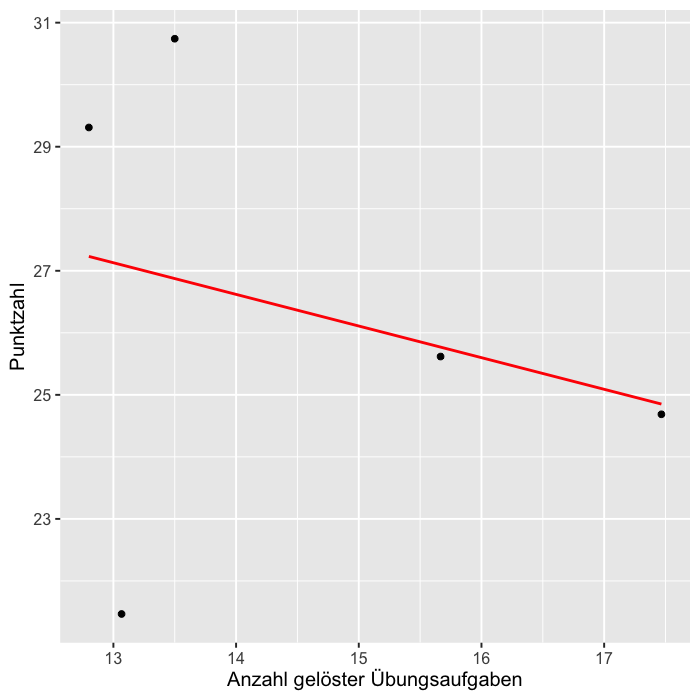
\includegraphics[width = 8cm, height = 8cm]{aggregation}
\caption{Zusammenhang zwischen der durchschnittlich gelösten Anzahl an Übungsaufgaben und der durschnittlich erreichten Punktzahl pro Klasse}
\label{fig:aggregiert}
\end{figure}

Die Analyse mittels Aggregation führt folglich nicht zu einem zufriedenstellenden Ergebnis und ist aufgrund der besprochenen Einschränkungen nicht geeignet, um Zusammenhänge auf Level-1 Ebene zu untersuchen.

\subsubsection{Disaggregation} \label{section:disaggregation}
Die zweite Möglichkeit um hierarchsiche Daten mit einem linearen Regressionsmodell zu untersuchen ist die Disaggregation. Wie bereits angedeutet werden bei der Disaggregation alle Level-2 Variablen auf Level-1 Einheiten verteilt. 

In unserem Beispiel werden also alle Schulkinder als von einander unabhängige Datenpunkte in die Analyse mit einbezogen. Dazu werden jedem Schulkind aus der selben Klasse die gleichen Werte der Level-2 Variablen zugeschrieben. In Tabelle \ref{tab:beispiel_theorie} aus Abschnitt \ref{section:bsp_theorie} kann man dieses Vorgehen bei den beiden Level-2 Variablen \textit{Klasse} und \textit{Fenster} beobachten. Durch diese Disaggregation von Level-2 Variablen auf Level-1 Einheiten werden Datensätze künstlich vergrössert und mögliche Variabilität, die zwischen den Level-2 Variablen besteht, wird ignoriert \citep{SnijdersTomA.B2012Ma:a, woltman2012introduction}. Folglich wird die geteilt Varianz zwischen Level-1 Einheiten nicht berücksichtigt und die Annahme, dass Fehler voneinander unabhängig sind, ist verletzt. Das führt dazu, dass die Effekte von Level-1 und Level-2 Variablen auf die abhängige Variable nicht voneinander getrennt werden können \citep{woltman2012introduction}. In unserem Beispiel würde das bedeuten, dass man den Einfluss der Anzahl an gelösten Übungsaufgaben nicht vom Einfluss der Klasse trennen kann. Ein weiteres Problem das durch Disaggregation entsteht, ist dass Abhängigkeiten innerhalb des Datensatzes unberücksichtigt bleiben \citep{woltman2012introduction}. Dies führt zu einer weiteren verletzten Annahme über die Unabhängigkeit von Beobachtungen. Die Verletzung dieser Annahme führt dazu, dass statistische Schätzer ungenau werden \citep{andrew_data, SnijdersTomA.B2012Ma:a, woltman2012introduction}.

\begin{figure}[t!]
\centering
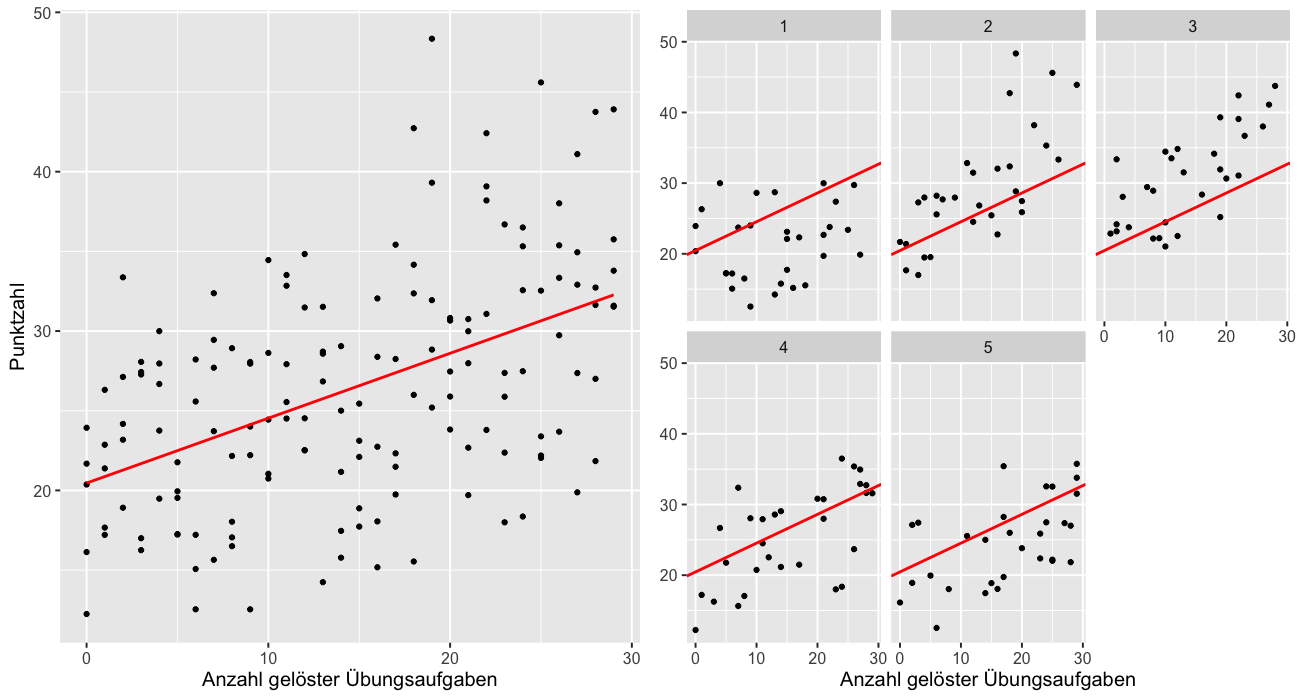
\includegraphics[width = \textwidth]{disaggregation_combined}
\caption{Zusammenhang zwischen der Anzahl gelöster Übungsaufgaben und erreichte Punktzahl mittels Disaggregation und Anwendung dieses Zusammenhangs auf jede der fünf Klassen}
\label{fig:disaggregation}
\end{figure}

Auf der linken Seite der Abbildung \ref{fig:disaggregation} befindet sich die Regressionsgerade, die durch ein lineares Regressionsmodell entsteht, wenn man mit einem disaggregierten Datensatz arbeitet. Anhand dieser Regressionsgerade besteht ein positiver Zusammenhang zwischen der Anzahl gelöster Übungsaufgaben und der erreichten Punktzahl in der Mathematikprüfung, so dass die erreichte Punktzahl mit steigender Anzahl an gelöster Übungsaufgaben zunimmt. Wie vorhin bereits erwähnt, wird in dieser Analyse aber nicht berücksichtigt, dass die Schulklasse selbst einen Effekt auf die erreicht Punktzahl haben kann. Dieser Effekt wird klar, wenn man die rechte Seite der Abbildung \ref{fig:disaggregation} betrachtet. Für jede der fünf Klassen wurde die selbe Regressionsgerade, die aus dem disaggregierten Datensatz entsteht, über die Daten gelegt. Man kann relativ einfach erkennen, dass es gewisse Klassen gibt, bei  denen mehr Schulkinder über oder unter der Regressionsgerade liegen. Des weiteren kann man erkennen, dass es nicht optimal ist, wenn für alle Klassen die selbe Steigung der Regressionsgerade verwendet wird. Betrachten wir beispielsweise die zweite Klasse, kann man erkennen, dass diese Schulkinder einen viel stärkeren Zusammenhang zwischen gelösten Übungsaufgaben und erreichter Punktzahl verzeichnen als die erste Klasse. Man könnte nun mit Hilfe einer Dummy-Kodierung den Einfluss von Klassen berücksichtigen, dazu müsste aber für jede Klasse einen zusätzlichen Parameter in das Modell aufgenommen werden. Da es grundsätzlich erstrebenswert ist, möglichst sparsame Modelle zu bilden ist auch dies keine optimale Lösung. Die Aggregation als auch die Disaggregation der Daten unterliegen massiven Einschränkungen und führen zu keinem zufriedenstellenden Ergebnis. Es erfordert folglich ein weiteres Modell, das Zusammenhänge innerhalb und zwischen Level-2 Einheiten abbilden kann ohne sich dabei auf eine Analyseinheit festzulegen.

\subsection{Hierarchische Linearen Modelle}
In den letzten Abschnitten wurde angenommen, dass sich die Regressionskoeffizienten $\beta_0$ und $\beta_1$ feste Werte sind, die sich nicht verändern. In Abbildung \ref{fig:disaggregation} aus dem vorherigen Abschnitt konnte man aber erkennen, dass diese Annahme nicht in allen Fällen zu einem erwünschten Ergebnis führt. In unserem Beispiel gibt es offensichtlich Klassen, die eine über- oder unterdurchschnittliche erreichte Punktzahl verzeichnen. Man kann nun annehmen, dass diese Regressionskoeffizienten zufällig sind. In diesem Kontext versteht man unter zufällig aber nicht, dass die Koeffizienten irgendwie gewählt werden können, sondern vielmehr, dass diese Koefizienten variieren können. 

In den folgenden Abschnitten werden nun hierarchische lineare Modelle besprochen, mit denen es möglich ist solche zufällige Koeffizienten zu schätzen. Als erstes wird das \textit{Random Intercept} Modell vorgestellt. Dieses Modell geht davon aus, dass die Höhe des Achsenabschnittes (\textit{intercept}) von der Gruppenzugehörigkeit abhängt und schätzt folglich mehrere verschiedene Achsenabschnitte. Das zweite besprochenen Modell ist das \textit{Random Intercept and Slope} Modell, bei dem sich nicht nur der Achsenabschnitt, sondern auch die Steigung (\textit{slope}) in Abhängigkeit der Gruppe unterscheidet. Dabei wird der Fokus vor allem darauf gesetzt, dass das Konzept von hierarchischen linearen Modellen verstanden wird. Wie genau solche HLMs mit R berechnet und analysiert werden, wird im Abschnitt \ref{section:ml_in_R} behandelt. 

\subsubsection{\textit{Random Intercept} Modell} \label{section:random_intercept_model}

Das \textit{Random Intercept} Modell ermöglicht es für jede Gruppe unterschiedliche Achsenabschnitte zu schätzen. Die einfachste Form eines \textit{Random Intercept} Modells ist ein Modell, das nur den Koeffizienten für den Achsenabschnitt $\beta_{0j}$ und das Residuum $\epsilon_i$ enthält. Dieses Modell wird wie folgt beschrieben:
\begin{equation}
\begin{split}	
\text{Level 1:} & \qquad y_{ji} 	= \beta_{0j} + \epsilon_{ij}\\
\text{Level 2:} & \qquad \beta_{0j} = \gamma_{00} + U_{0j}
\end{split}	
\end{equation} 
Bei dieser Darstellung handelt es sich um die hierarchische Notation der Gleichung, da die einzelnen Gleichungen gleich dem dazugehörigen Level zugeordnet werden. Dies wird klarer, wenn man es in Bezug zu unserem Beispiel betrachtet. Auf Level-1 befindet sich die Regressionsgleichung für die erreichte Punktzahl jedes einzelnen Schulkindes $i$ aus der Klasse $j$. Dabei kann man erkennen, dass der Regressionskoeffizient $\beta_{0j}$ von der Klasse $j$ abhängt und folglich für jede Klasse einen anderen Wert einnimmt. Da die Klasse eine Level-2 Variable ist, befindet sich die Gleichung für $\beta_{0j}$ auf Level-2. Dabei ist $\gamma_{00}$ der Gesamtmittelwert und $U_{0j}$ die zufällige Abweichung der Klasse $j$ vom Gesamtmittelwert. Substituiert man die Gleichung von Level-2 in die Gleichung von Level-1 gelangt man zur flachen Notation dieses \textit{Random Interceot} Modells:
\begin{equation}
\begin{split}
y_{ji} 	& = \beta_{0j} + \epsilon_{ij}\\
		& = \gamma_{00} + U_{0j} + \epsilon_{ij}
\end{split}
\end{equation}
Diese Gleichung entspricht dem leeren Modell aus Abschnitt \ref{section:icc}, anhand dessen man die Intraklassen Korrelation berechnet. Ähnlich wie bei der normalen linearen Regression können diesem Modell nun weitere Variablen hinzugefügt werden, um die Varianz in der erreichten Punktzahl des Schulkindes $i$ aus der Klasse $j$ zu erklären. In unserem Beispiel ergänzen wir das Modell mit nur einer weiteren Varialbe $x_{ij}$, die der Anzahl gelöster Übungsaufgaben entspricht:
\begin{equation} \label{eq:random_intercept_model}
\begin{split}	
 \text{Level 1:}  	\qquad 	y_{ji} 		& = \beta_{0j} + \beta_{1}x_{ij} + \epsilon_{ij}\\
 \text{Level 2:} 	\qquad 	\beta_{0j} 	& = \gamma_{00} + U_{0j}\\
 							\beta_{1} 	& = \gamma_{10}
\end{split}	
\end{equation} 
Da es sich hier um ein \textit{Random Interceot} Modell handelt, bleibt die Steigung für alle Klassen gleich. Dies kann man an der Gleichung des Koeffizienten $\beta_{1}$ erkennen, da es keine zufällige Abweichung in Abhängigkeit der Klasse $j$ von der Gesamtsteigung $\gamma_{10}$ gibt. Werden nun aus \eqref{eq:random_intercept_model} die beiden Gleichungen auf Level-2 in die Gleichung auf Level-1 eingesetzt, gelangen wir wieder zur flachen Notation des \textit{Random Intercept} Modells:
\begin{equation}
\begin{split}
y_{ji} 	& = \beta_{0j} + \beta_{1}x_{ij} + \epsilon_{ij} \\
		& = \gamma_{00} + U_{0j} + \gamma_{10}x_{ij} + \epsilon_{ij} \\
		& = \gamma_{00} + \gamma_{10}x_{ij} + U_{0j} + \epsilon_{ij}
\end{split}
\end{equation}

In Abbildung \ref{fig:random_intercept} kann man nun die Graden für jede einzelne Klasse erkennen. Die rote Gerade entspricht der linearen Regressionsgerade, die durch die Disaggregation entsteht und wird hier als Vergleichswert zu den anderen Geraden verwendet. Auf der linken Seite der Abbildung erkennt man relativ schnell, dass es bedeutende Unterschiede zwischen den Klassen gibt. Werden die Geraden für jede einzelne Klasse betrachtet, erhält man einen Überblick über das Leistungslevel der verschiedenen Klassen. Beispielsweise kann man erkennen, dass die Klassen eins und fünf eher tiefere und die Klassen zwei und drei eher höhere Punktzahlen erreichen. Diese Unterschiede kommen durch die unterschiedliche Ausprägungen der zufälligen Abweichungen $U_{0j}$ zustande. Für die Klasse 3 ergibt sich beispielsweise aus unserem \textit{Random Intercept} Modell einen Schätzer für die zufällige Abweichung von $U_{03} = 4.54$ und für den Gesamtmittelwert $\gamma_{00} = 19.9$. Setzt man diese beiden Werte in die Gleichung aus \eqref{eq:random_intercept_model} erhält man den klassenspezifischen Achsenabschnitt $\beta_{03}$:
\begin{equation}
\beta_{03} = 19.9 + 4.54 = 24.43
\end{equation} 
Schulkinder der Klasse 3 erreichen bei $0$ gelösten Übungsaufgaben im Mittel eine Punktzahl von $24.43$. Für Klasse 1 lässt sich ihr Achsenabschnitt $\beta_{01}$ genau gleich bestimmen. Aus der klassenspezifischen Abweichung $U_{01} = -4.01$ und dem Gesamtmittelwert von $\gamma_{00} = 19.9$ ergibt sich ein Achsenabschnitt von $\beta_{01} = 15.89$. Schulkinder aus Klasse eins erreichen bei 0 gelösten Übungsaufgaben im Mittel also eine tiefere Punktzahl als Schulkinder aus Klasse 3. Diese Aussage stimmt ebenfalls mit den Geraden aus Abbildung \ref{fig:random_intercept} überein. Das Prinzip des Zusammenhangs zwischen der zufälligen Abweichung $U_{0j}$ und dem Gesamtmittelwert $\gamma_{00}$ kann also ähnlich wie bei einer Dummy-Kodierung verstanden werden. Dabei ist der Gesamtmittelwert die Referenzkategorie, von der jede Klasse um $U_{0j}$ abweicht.

\begin{figure}[t!]
\centering
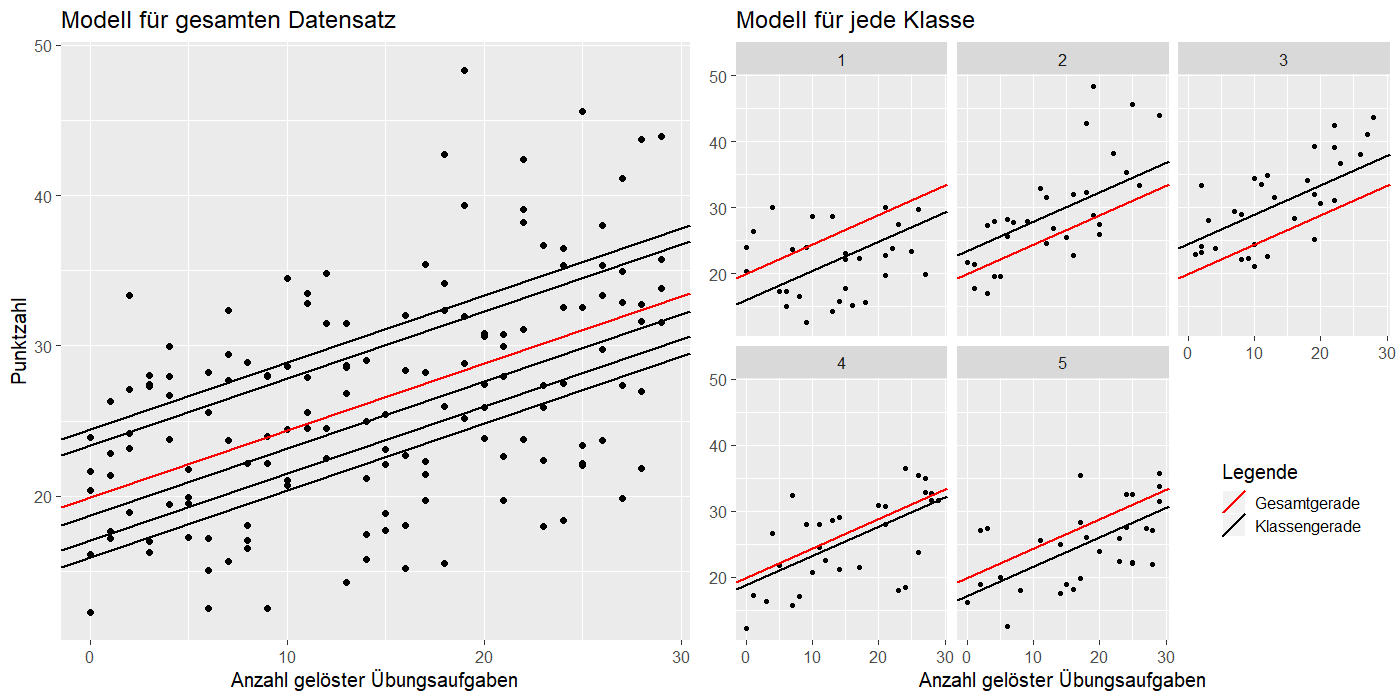
\includegraphics[width = \textwidth]{random_intercept}
\caption{Zusammenhang zwischen der Anzahl gelöster Übungsaufgaben und der erreichten Punktzahl unter Berücksichtigung der Klassenzugehörigkeit}
\label{fig:random_intercept}
\end{figure}

Ebenfalls kann man beobachten, dass die Geraden des hierarchischen linearen Modells besser zu den Daten passen. Dies wird etwas klarer, wenn man die Residuenplots des \textit{Random Intercept} Modells und des normalen linearen Modells vergleicht. In Abbildung \ref{fig:resid_lm_rim} sind die beiden Residuenplots abgebildet. Auch wenn die Unterschiede nicht all zu gross sind, kann man erkennen, dass es beim \textit{Random Intercept} Modell weniger grosse Abweichungen gibt zwischen den tatsächlich beobachteten Werten und den vom Regressionsmodell erwarteten Werten. Allerdings fällt beim Residuenplot des \textit{Random Intercept} Modells auf, dass an den Endpunkten die Residuen nicht mehr um den Nullpunkt verteilt sind, beim linearen Modell allerdings schon. Die Ursache dafür besteht darin, dass die Residuen nun für jede einzelne Regressionsgerade der Klassen berechnet werden. Da bei dem normalen linearen Modell die Residuen alle nur an einer Geraden berechnet werden, gleichen sich die Residuen der Schulkinder aus leistungsstärkeren Klassen mit den Kindern aus leistungsschwächeren Klassen aus. Betrachtet man in Abbildung \ref{fig:random_intercept} die rechte Seite, passen die Regressionsgeraden des \textit{Random Intercept} Modells besser zu den Daten als das lineare Modell. Allerdings gibt es immer noch Schulkinder, die noch nicht optimal durch die Gerade beschrieben werden. Bei der zweiten und dritten Klasse erreichten beispielsweise Schulkinder, die viele Übungen gelöst haben eine noch viel höhere Punktzahl als vom Modell angenommen wird. Diese Ungenauigkeit führt folglich zu einer unpassenden Verteilung der Residuen an den Endpunkten. Anscheinend gibt es in unserem Datensatz Klassen, bei denen die Schulkinder einen stärkeren oder schwächeren Anstieg der erreichten Punktzahl bei steigender Anzahl gelöster Übungsaufgaben verzeichnen. Daraus könnte man nun folgern, dass sich nicht nur der Achsenabschnitt zwischen den Klassen unterscheidet, sondern auch die Steigung.

\begin{figure}[t!]
\centering
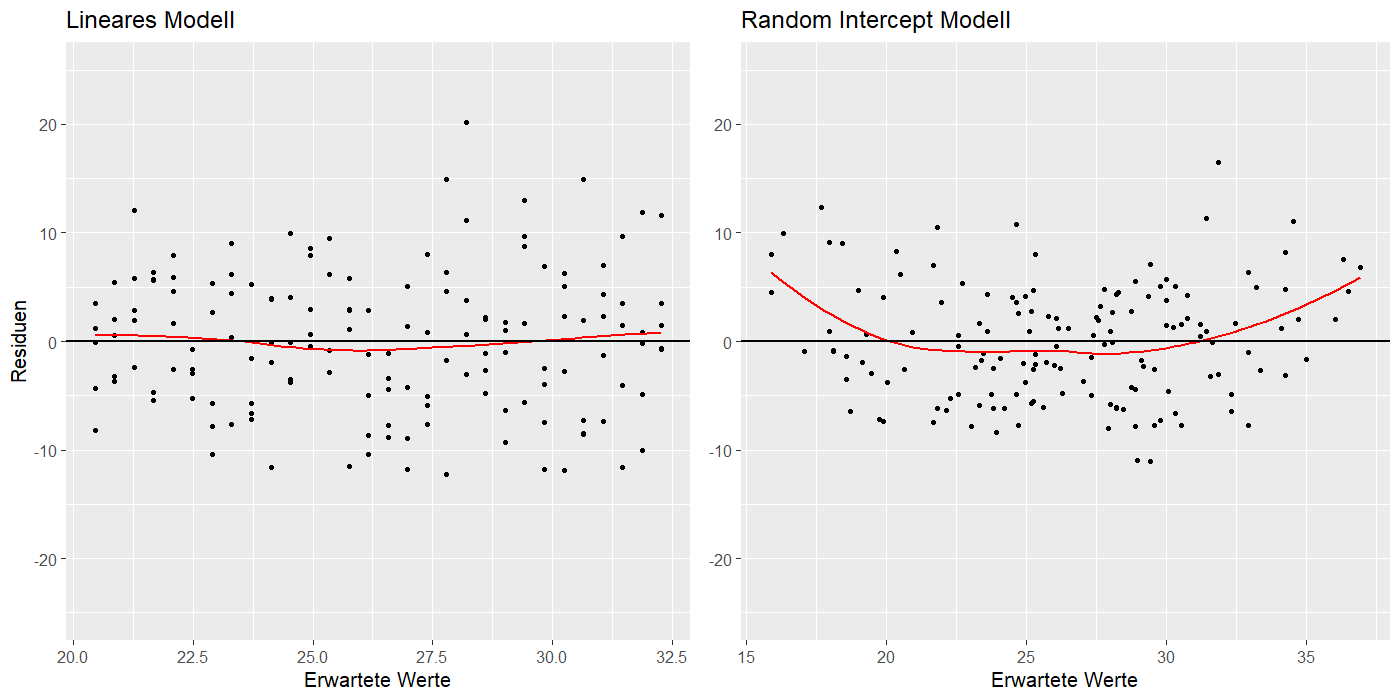
\includegraphics[width = \textwidth]{residuen_lm_rim}
\caption{Residuenplot des linearen Modells und des \textit{Random Intercept} Modells}
\label{fig:resid_lm_rim}
\end{figure}

\subsubsection{\textit{Random Intercept and Slope} Modell} \label{section:random_intercept_slope_model}

Im letzten Abschnitt wurde das \textit{Random Intercept} Modell besprochen und aufgezeigt, dass man durch die Hinzunahme von variierenden Achsenabschnitten eine bessere Passung zwischen dem Modell und den Daten erreicht. Um eine noch bessere Passung zu erreichen und genauere Vorhersagen zu treffen kann man nun nicht nur den Achsenabschnitt, sondern auch die Steigung variieren lassen. Dies führt zum \textit{Random Intercept and Slope} Modell, das die Interaktion zwischen Klassenzugehörigkeit und der Anzahl gelöster Übungsaufgabe berücksichtigt. Der Regressionskoeffizient $\beta_{1}$ aus dem \textit{Random Intercept} Modell \eqref{eq:random_intercept_model} ist nun von der Klasse $j$ abhängig und wird durch die zufällige Abweichung $U_{1j}$ erweitert. Dies führt zum folgenden Modell in der hierarchischen Notation:
\begin{equation} \label{eq:random_intercept_slope_model}
\begin{split}	
 \text{Level 1:}  \qquad y_{ji} & = \beta_{0j} + \beta_{1}x_{ij} + \epsilon_{ij}\\
 \text{Level 2:} \qquad \beta_{0j} & = \gamma_{00} + U_{0j}\\
 \beta_{1j} & = \gamma_{10} + U_{1j}
\end{split}	
\end{equation} 
Durch Einsetzen und Umformen erhalten wir wieder die flache Notation unseres Modells:
\begin{equation} \label{eq:flat_random_intercept_slope_model}
\begin{split}	
y_{ji} & = \beta_{0j} + \beta_{1}x_{ij} + \epsilon_{ij}\\
& = \gamma_{00} + U_{0j} + (\gamma_{10} + U_{1j})x_{ij} + \epsilon_{ij}\\
& = \gamma_{00} + \gamma_{10}x_{ij} + U_{0j} + U_{1j}x_{ij} + \epsilon_{ij}
\end{split}	
\end{equation} 
Dabei wurde die Gleichung so umgeformt, dass der erste Teil $\gamma_{00} + \gamma_{10}x_{ij}$ die jeweiligen Gesamtmittelwerte enthält. Diese Werte sind unveränderbar und werden folglich als fester Teil des Modells bezeichnet. Der zweite Teil der Gleichung mit $U_{0j} + U_{1j}x_{ij} + \epsilon_{ij}$ wird als zufälliger Teil bezeichnet, weil er alle veränderbaren Werte enthält. Der Term $U_{1j}x_{ij}$ beschreibt die zufällige Interaktion zwischen Gruppenzugehörigkeit und der Variable $x_{ij}$. Bezogen auf unser Beispiel bedeutet dieser Term, wie stark und in welche Richtung sich die erreichte Punktzahl verändert in Abhängigkeit der Klassenzugehörigkeit und der Anzahl gelöster Übungen. 
\begin{figure}[ht!]
\centering
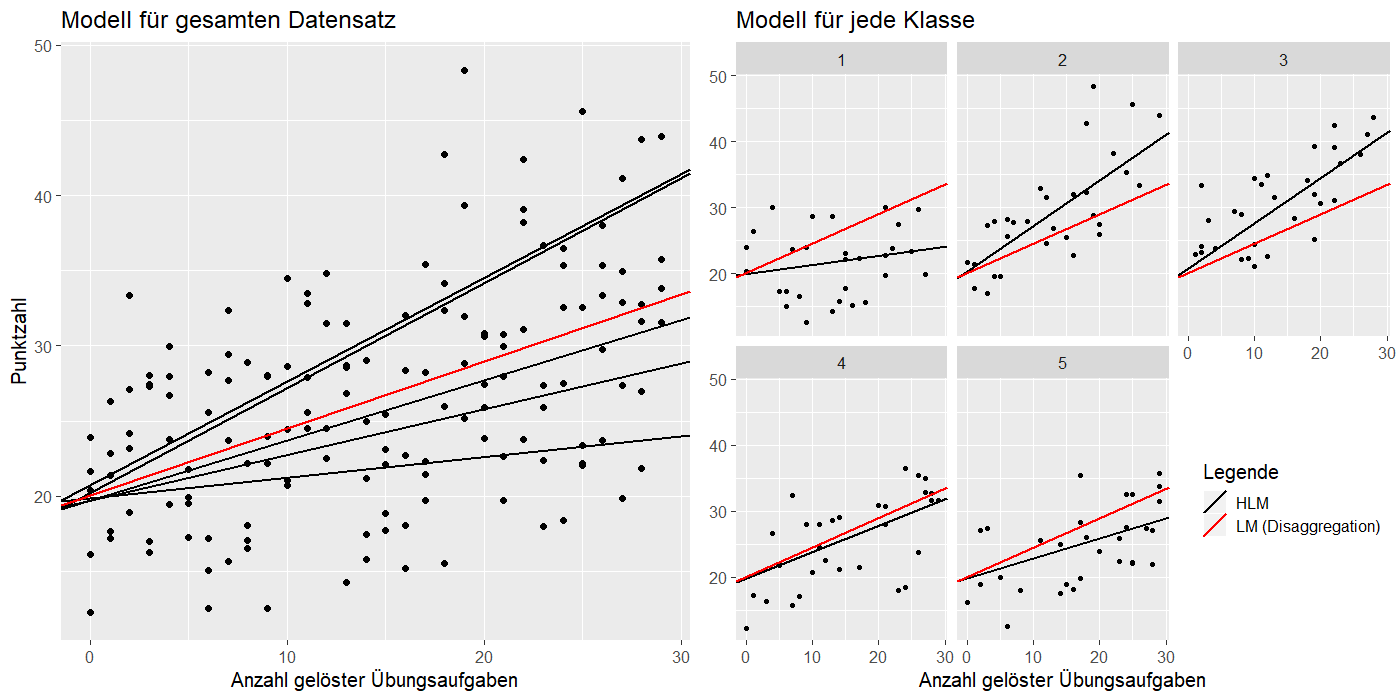
\includegraphics[width = \textwidth]{random_intercept_slope}
\caption{Zusammenhang zwischen der Anzahl gelöster Übungsaufgaben und der erreichten Punktzahl unter Berücksichtigung der Klassenzugehörigkeit und deren Interaktion mit der Anzahl gelöster Übungsaufgaben}
\label{fig:random_intercept_slope}
\end{figure}
In Abbildung \ref{fig:random_intercept_slope} ist diese zufällige Interaktion einfach zu erkennen. Für gewisse Klassen nimmt die Zufallsvariable $U_{1j}$ eine positiven und für andere einen negativen Wert ein. Dies spiegelt sich wiederum in klassenspezifischen Steigungen $\beta_{1j}$ die höher oder tiefer als die mittlere Steigung $\gamma_{10}$ sind. Betrachten wir die Klasse 3 unseres Beispiels. Das \textit{Random Intercept and Slope} Modell schätzt für diese Klasse eine zufällige Abweichung $U_{13} = 0.22$ von der mittleren Steigung $\gamma_{10} = 0.45$. Setzt man nun diese beide Werte in die Gleichung für $\beta_{1j}$ aus \eqref{eq:random_intercept_slope_model} ein erhält man die klassenspezifische Steigung $\beta_{13}$.
\begin{equation} \label{eq:beta1_example}	
\beta_{13} = 0.45 + 0.22 = 0.67
\end{equation} 
Für jede weitere gelöste Übungsaufgabe eines Schulkindes $j$ aus der Klasse 3 steigt also die erwartete Punktzahl im Mittel um $0.67$ Punkte an. Betrachten wir nun die Klasse 1 aus unserem Beispiel, schätzt unser Modell eine negative zufällige Abweichung $U_{11} = -0.24$ von der mittleren Steigung. Wird dieser Wert wieder in die Gleichung für $\beta_{1j}$ aus \eqref{eq:random_intercept_slope_model} eingesetzt, erhalten wir einen klassenspezifische Steigung von $\beta_{11} = 0.2$. Diese Steigung ist nun kleiner als die mittlere Steigung aller Klassen $\gamma_{10} = 0.45$. Folglich nimmt die erreichte Punktzahl bei einer weiteren gelösten Übungsaufgabe eines Schulkindes $j$ aus der Klasse 1 im Mittel nur um $0.2$ zu. 

In unserem Beispiel ist es also so, dass je höher der klassenspezifische Achsenabschnitt ist, desto höher ist auch die klassenspezifische Steigung Steigung. Man spricht hier auch von einer positiven Korrelation zwischen Achsenabschnitt und Steigung. Diese beiden Koeffizienten müssen aber nicht zwingend positive miteinander korreliert sein. Es gibt auch die Möglichkeit, dass diese Koeffizienten negativ korreliert oder sogar unkorreliert sind. In Abbildung \ref{fig:corr_s_i} kann man betrachten, wie die weiteren Korrelationen von Achsenabschnitt und Steigung sich auswirken. Bei einer negativen Korrelation nimmt die Steigung mit der Höhe des Achsenabschnittes ab. Sind die beiden Koeffizienten unkorreliert, bildet sich kein offensichtliches Muster zwischen der Höhe des Achsenabschnittes und der Steigung.

\begin{figure}[ht!]
\centering
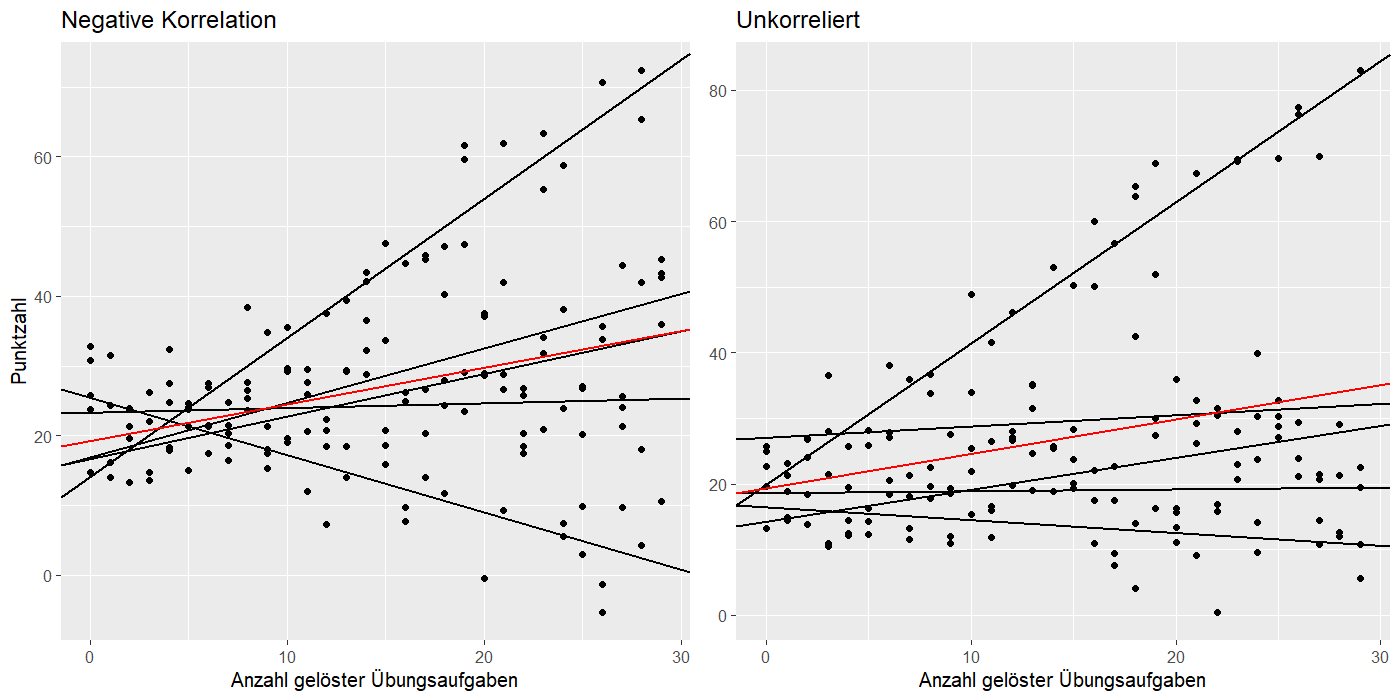
\includegraphics[width = \textwidth]{corr_s_i}
\caption{Darstellung einer negativen und nicht vorhandenen Korrelationen zwischen Achsenabschnitt und Steigung}
\label{fig:corr_s_i}
\end{figure}

In Abschnitt \ref{section:random_intercept_model} wurden die Residuenplots eines linearen Modells und eines \textit{Random Intercept} Modells verglichen. Dabei ist aufgefallen, dass das \textit{Random Intercept} Modell zwar kleinere Residuen aufwies, diese aber an den Endpunkten nicht um den Nullpunkt normalverteilt waren. Vergleicht man nun den Residuenplot aus Abbildung \ref{fig:resid_rism} mit den anderen aus der Abbildung \ref{fig:resid_lm_rim}, hat sich die Lage bezüglich der Verteilung der Residuen an den Endpunkten deutlich verbessert im \textit{Random Intercept and Slope} Modell.
 
\begin{figure}[ht!]
\centering
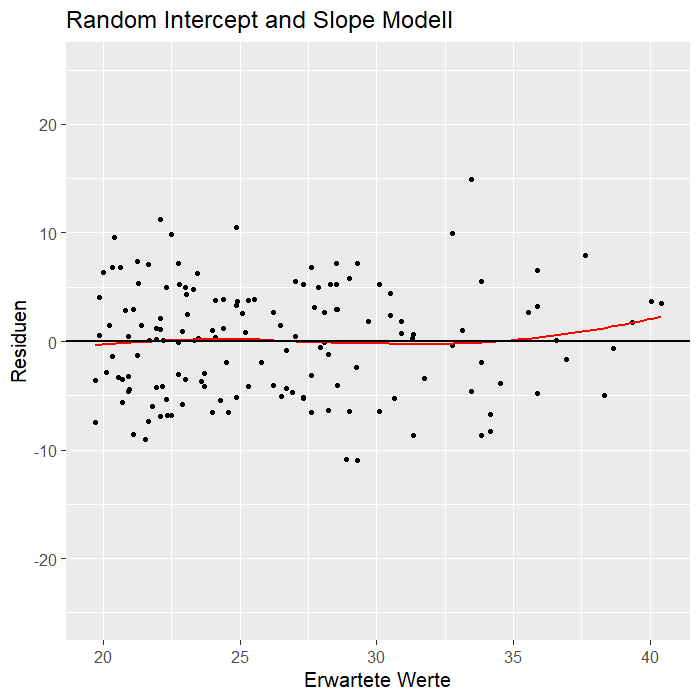
\includegraphics[width = 8cm, height = 8cm]{residuen_rism}
\caption{Residuenplot des \textit{Random Intercept and Slope} Modells}
\label{fig:resid_rism}
\end{figure}

\subsubsection{\textit{Intercept} und \textit{Slope} Variabilität} \label{section:variability}
Wie bei linearen Regressionsmodellen wird auch bei hierarchsichen linearen Regressionsmodellen versucht die Variabilität einer bestimmten Abhängigen Variablen zu erklären. Diese unerklärte Variabilität hängt in hierarchischen linearen Modellen nicht nur von der Varianz des Residuums $\epsilon_{ij}$ ab, sondern auch von der Varianz der zufälligen Abweichung des Achsenabschnittes $U_{0j}$ und der Steigung $U_{1j}$ \citep{SnijdersTomA.B2012Ma:a}. Um nun unerklärte Variabilität in hierarchischen Modellen zu beschreiben, können alle dieser Komponenten angegangen werden. Um die Varianz des Residuums zu verringern können, wie bei der normalen linearen Regression, weitere Level-1 Variablen in das Modell aufgenommen werden. Um die Varianz der beide zufälligen Abweichungen zu verringern wird es etwas anspruchsvoller, da diese beiden Varianzen nicht durch Unterschieden innerhalb der Gruppen sondern zwischen den Gruppen entstehen. Folglich können diese Varianzen nicht durch das Hinzufügen von Level-1 Variablen reduziert werden, sondern erfordern das Hinzufügen von Level-2 Variablen. Snijders und Bosker \citeyearpar{SnijdersTomA.B2012Ma:a} erweitern hierfür die beiden Gleichungen für die Regressionskoeffizienten $\beta_{0j}$ und $\beta_{1j}$:
\begin{equation} \label{eq:variance}
\begin{split}	
 \text{Level 1:}  \qquad y_{ji} & = \beta_{0j} + \beta_{1}x_{ij} + \epsilon_{ij}\\
 \text{Level 2:} \qquad \beta_{0j} & = \gamma_{00} + \gamma_{01}z_{j} + U_{0j}\\
 \beta_{1j} & = \gamma_{10} + \gamma_{11}z_{j} + U_{1j}
\end{split}	
\end{equation}
Dabei ist $z_{j}$ eine Level-2 Variable, die sich zwischen den Gruppen unterscheidet. Auf unser Beispiel bezogen, könnte die Variable $z_{j}$ die Anzahl Fenster im Klassenzimmer sein. Durch das Hinzufügen dieser Level-2 Variablen werden die Regressionskoeffizienten selbst zu einer Abhängigen Variablen eines Regressionmodells. Setzt man nun die beiden Koeffizienten in die Level-1 Gleichung ein erhält man wieder die flache Notation des Modells:
\begin{equation} \label{eq:flat_variance}
\begin{split}	
y_{ji} & = \beta_{0j} + \beta_{1}x_{ij} + \epsilon_{ij}\\
& = \gamma_{00} + \gamma_{01}z_{j} + U_{0j} + (\gamma_{10} + \gamma_{11}z_{j} + U_{1j})x_{ij} + \epsilon_{ij}\\
& = \gamma_{00} + \gamma_{01}z_{j} + U_{0j} + \gamma_{10}x_{ij} + \gamma_{11}z_{j}x_{ij} + U_{1j}x_{ij} + \epsilon_{ij}\\
& = \gamma_{00} + \gamma_{01}z_{j} + \gamma_{10}x_{ij} + \gamma_{11}z_{j}x_{ij} + U_{0j} + U_{1j}x_{ij} + \epsilon_{ij}\\
\end{split}	
\end{equation} 
Auch wenn es in der hierarchischen Notation einfacher ist zu erkennen, welche Varianz genau durch die Hinzunahme dieser Level-2 Variable verringert wird, erkennt man in der flachen Notation einen weiteren wichtigen Zusammenhang. Der Term $\gamma_{11}z_{j}x_{ij}$ beschreibt eine besondere Interaktion zwischen einer Level-1 und einer Level-2 Variable und wird, wie bereits in der Einleitung kurz erwähnt, als \textit{Cross-Level} Interaktion bezeichnet. Da diese \textit{Cross-Level} Interaktion durch das Hinzufügen einer Level-2 Variable als Prädiktor in der Gleichung des Steigungskoeffizienten entsteht, ist diese Interaktion vor allem wichtig, um unerklärte Varianz in der Steigung zu erklären. In unserem Beispiel würde diese \textit{Cross-Level} Interaktion also durch die Interaktion zwischen der Anzahl gelösten Übungsaufgaben und der Anzahl Fenster im Klassenzimmer beschreiben werden.

In den letzten Abschnitten wurden zwei verschiedene hierarchische lineare Modelle besprochen und das Prinzip ihrer Anwendung etwas näher gebracht. Es ist dabei zu berücksichtigen, dass hier nur die Grundlagen zu den hierarchischen linearen Modellen behandelt wurden. Für eine weitere Vertiefung dieses Themas wird auf die gängige Literatur zur Multilevel Analyse verwiesen \citep{andrew_data, SnijdersTomA.B2012Ma:a, twisk_2006}. Im anschliessenden Kapitel geht es nun darum, wie man genau solche Modelle in R berechnet und Multilevel Analysen durchführt.

\subsection{Anwendung von Multilevel Analyse in R} \label{section:ml_in_R}
Das Konzept von hierarchischen linearen Modellen wurde in den letzten Abschnitten ausführlich besprochen. In den nächsten Abschnitten wird vor allem die Anwendung dieser Modelle behandelt. Dabei wird der Fokus auf die Programmiersprache R gelegt und dessen Zusatzpaket \texttt{lme4} \citep{batesetal2015lme4}, das neben weiteren Paketen die Analyse mittels HLMs ermöglicht. Dabei wird davon ausgegangen, dass die Grundlagen dieser Programmiersprache verstanden wurden. Zuerst werden allgemeine Informationen und die Syntax von \texttt{lme4} besprochen. Anschliessend wird anhand unseres Beispiels ein erstes Modell geschätzt und dessen \texttt{summary()}-Output interpretiert. Dabei werden noch weitere Möglichkeiten besprochen, wie man Ergebnisse eines Geschätzten Modells präsentieren kann. Nachdem die Syntax und Interpretation des Modells besprochen wurden, wird Schritt für Schritt eine Multilevel Analyse unseres Beispiels durchgeführt. Hierbei wird aufgezeigt, wie HLMs aufgebaut und miteinander verglichen werden, um das geeignetste Modell zu identifizieren. Am Ende dieses Abschnittes werden Effektsterkemasse besprochen, die bei der Auswertung und Berichterstattung von HLMs wichtig sind.  

\subsubsection{Informationen und Syntax von \texttt{lme4}}
Mit dem Paket \texttt{lme4} lassen sich verschiedenste Formen von hierarchischen Modellen schätzen und analysieren. Dabei werden wir uns hier hauptsächlich auf die Funktion \texttt{lmer()} beschränken. Diese Funktion wird verwendet, um hierarchische lineare Modelle zu schätzen und dessen Syntax ist relativ ähnlich mit der Syntax des Befehls für die Berechnung normaler linearer Modelle \texttt{lm()}. Sie ist wie folgt aufgebaut:

\begin{knitrout}
\definecolor{shadecolor}{rgb}{0.969, 0.969, 0.969}\color{fgcolor}\begin{kframe}
\begin{alltt}
\hlkwd{lmer}\hlstd{(formula, data, REML)}
\end{alltt}
\end{kframe}
\end{knitrout}

Dabei wird in \texttt{formula} die gewünschte Formel des Modells eingegeben, bei \texttt{data} wird der Datensatz festgelegt anhand das Modell geschätzt werden soll und bei \texttt{REML} wird durch einen logischen Operator (\textit{TRUE} oder \textit{FALSE}) eingestellt, ob das Modell mit \textit{Restricted Maximum Likelihood} (REML) oder mit \textit{Maximum Likelihood} (ML) geschätzt werden soll. In unserem Fall ist diese Einstellung vor allem beim Vergleich von Modellen wichtig. Bei Modellen die mit REML geschätzt wurden, können nur die zufälligen Effekte miteinander verglichen werden. Wenn man also feste als auch zufällige Effekte vergleichen möchte, sollte man Modelle mit ML schätzen \citep{PEUGH201085}. 

\begin{knitrout}
\definecolor{shadecolor}{rgb}{0.969, 0.969, 0.969}\color{fgcolor}\begin{kframe}
\begin{alltt}
\hlkwd{lmer}(Abhängige Variable ~ Feste Effekte + (Zufällige Effekte | Gruppe), ... )
\end{alltt}
\end{kframe}
\end{knitrout}

Bis zum Term innerhalb der Klammer ist die Syntax von \texttt{lmer()} genau die gleiche wie bei \texttt{lm()}. Dabei wird auf zuerst die zu erklärende Variable aufgeführt und anschliessend alle Variablen, die als feste Effekte in das Modell aufgenommen werden sollen. Innerhalb der Klammern können nun die zufälligen Effekte und die variierende Gruppe festgelegt werden. Dabei kann innerhalb der Klammern eingestellt werden, ob der Achsenabschnitt und die Steigung korrelieren sollten oder nicht. In Tabelle \ref{tab:lmersyntax} findet man einen Überblick über die möglichen Interaktionen, die man innerhalb der Klammer festlegen kann und die für uns relevant sind\footnote{Weitere Funktionen und eine ausführliche Beschreibung des Paketes \texttt{lme4} können in Bates et al. \citeyearpar{batesetal2015lme4} nachgeschlagen werden.}.
\begin{table}[ht] 
\centering
\caption{Mögliche Syntax für \texttt{lmer()} nach Bates et al. \citeyearpar{batesetal2015lme4}}
\begin{tabular}{ll}
 	\toprule
	Formel & Bedeutung\\ 
  	\midrule
	(1 $|$ Gruppe)	& Zufälliger Achsenabschnitt \\
	(x $|$ Gruppe) & Korrelierter Achsenabschnitt und Steigung \\
	(x $||$ Gruppe) & Unkorrelierter Achsenabschnitt und Steigung\\
  	\bottomrule
\end{tabular}
\label{tab:lmersyntax}
\end{table}

\subsubsection{Interpretation eines Outputs} \label{section:interpretation_output}
Wir haben nun den groben Aufbau von \texttt{lmer()} besprochen und schätzen nun ein erstes Modell. Dafür muss zuerst das Paket \texttt{lme4} und unser Beispieldatensatz geladen werden.

\singlespacing
\begin{knitrout}
\definecolor{shadecolor}{rgb}{0.969, 0.969, 0.969}\color{fgcolor}\begin{kframe}
\begin{alltt}
\hlkwd{library}\hlstd{(lme4)}
\hlstd{beispiel_data} \hlkwb{<-} \hlkwd{readRDS}\hlstd{(}\hlkwc{file} \hlstd{=} \hlstr{"dataset_theory"}\hlstd{)}
\end{alltt}
\end{kframe}
\end{knitrout}
\setstretch{1.5}

Anschliessend wird ein Modell mit der Anzahl gelösten Übungen als fester Effekt und mit variierenden Achsenabschnitten und Steigungen geschätzt und mittels \texttt{summary()} übersichtlich ausgegeben.

\singlespacing
\begin{knitrout}
\definecolor{shadecolor}{rgb}{0.969, 0.969, 0.969}\color{fgcolor}\begin{kframe}
\begin{alltt}
\hlstd{beispiel_model} \hlkwb{<-} \hlkwd{lmer}\hlstd{(punktzahl} \hlopt{~} \hlstd{uebung} \hlopt{+} \hlstd{(uebung} \hlopt{|} \hlstd{klasse),}
    \hlkwc{data} \hlstd{= beispiel_data,} \hlkwc{REML} \hlstd{=} \hlnum{FALSE}\hlstd{)}
\hlkwd{summary}\hlstd{(beispiel_model)}
\end{alltt}
\begin{verbatim}
## Linear mixed model fit by maximum likelihood  ['lmerMod']
## Formula: punktzahl ~ uebung + (uebung | klasse)
##    Data: beispiel_data
## 
##      AIC      BIC   logLik deviance df.resid 
##      944      963     -466      932      144 
## 
## Scaled residuals: 
##     Min      1Q  Median      3Q     Max 
## -2.1080 -0.8358  0.0364  0.7288  2.9172 
## 
## Random effects:
##  Groups   Name        Variance Std.Dev. Corr
##  klasse   (Intercept)  0.9191  0.959        
##           uebung       0.0349  0.187    1.00
##  Residual             26.5996  5.157        
## Number of obs: 150, groups:  klasse, 5
## 
## Fixed effects:
##             Estimate Std. Error t value
## (Intercept)  19.9971     0.9360   21.36
## uebung        0.4481     0.0973    4.61
## 
## Correlation of Fixed Effects:
##        (Intr)
## uebung 0.000 
## convergence code: 0
## boundary (singular) fit: see ?isSingular
\end{verbatim}
\end{kframe}
\end{knitrout}
\setstretch{1.5}

Dabei kann man im Output direkt die geschätzten Werte für die zufälligen und festen Effekte ablesen. Bei den zufälligen Effekten werden für den Achsenabschnitt als auch für die Steigung die geschätzte Varianzen, die Standardabweichungen, als auch die Korrelation dieser beiden angegeben. Ebenfalls werden direkt unterhalb der zufälligen Effekte aufgeführt wie gross die verwendete Stichprobe war und wie viele Gruppen für die Schätzung verwendet wurden. In unserem Fall waren das 150 Schulkinder, verteilt auf 5 Klassen. Der Abschnitt zu den festen Effekten ähnelt stark dem Output der Funktion \texttt{lm()} und lässt sich auch dementsprechend interpretieren. Es werden hier aber keine $p$-Werte angezeigt, da man sich in der Forschung noch uneinig darüber ist, wie genau die Anzahl der Freiheitsgrade geschätzt werden soll \citep{PEUGH201085,SnijdersTomA.B2012Ma:a}\footnote{Möchte man $p$-Werte anzeigen lassen, kann man das mit dem Paket \texttt{lmerTEST} \citep{lmertest}.}. Eine Interpretation des Achsenabschnittes unter Berücksichtigung der zufälligen Effekte würde dann wie folgt lauten: 
\begin{quote}
Die erwartete erreichte Punktzahl in der Mathematikprüfung ist $19.99 \pm 2 \cdot 1.07$ Punkte, wenn keine einzige Übungsaufgabe gelöst wurde.
\end{quote}
Und für die Steigung:
\begin{quote}
Die erwartete Zunahme der Punktzahl beträgt $0.45 \pm 2 \cdot 0.21$ pro gelöste Übungsaufgabe.
\end{quote}
Dabei ist 1.07 die Standardabweichung des Achsenabschnittes und 0.21 die Standardabweichung der Steigung. Bei der Interpretation ist es von Vorteil die Standardabweichung zu verwenden, da diese nicht wie die Varianz quadriert ist und somit der Masseinheit (Punktzahl) entspricht. 

\subsubsection{Berechnung der Intraklassen Korrelation in R} \label{section:icc_r}
Wir gelangen nun zur Analyse unseres Beispieldatensatzes. Bevor wir mit der Analyse starten können ist es wichtig, dass wir das Level unserer Forschungsfrage klar definieren. In unserem Fall möchten wir herausfinden, wie genau sich die Prüfungsleistung von Schulkindern mit der Anzahl gelöster Übungsaufgaben unter Berücksichtigung der Klassenzugehörigkeit verändert. Das bedeutet, dass sich unsere abhängige Variable auf Level-1 befindet. Ebenfalls sollte berücksichtigt werden, dass es zu Interaktionen zwischen Level-1 und Level-2 variablen kommen kann. Da wir sehr wahrscheinlich nicht nur feste Effekte sondern auch zufällige Effekte miteinander Vergleichen möchten, müssen wir zudem die Modelle mit ML schätzen \citep{PEUGH201085}. 

Als Erstes sollte immer geprüft werden, ob eine Multilevel Analyse überhaupt nötig ist. Dies geschieht zum einen durch die Berechnung der Intraklassen Korrelation und der Überprüfung, ob überhaupt mittlere Unterschiede zwischen den Klassen bestehen. Wie bereits im Abschnitt \ref{section:icc} besprochen, lässt sich die IKK aus den Varianzen des leeren Modells berechnen, das hier noch einmal kurz aufgeführt ist:
\begin{equation}
\begin{split}	
 \text{Level 1:}  \qquad y_{ji} & = \beta_{0j} + \epsilon_{ij}\\
 \text{Level 2:} \qquad \beta_{0j} & = \gamma_{00} + U_{0j}\\
\end{split}	
\end{equation} 
Dieses Modell wird wie folgt in R mittels der Funktion \texttt{lmer()} geschätzt:

\singlespacing
\begin{knitrout}
\definecolor{shadecolor}{rgb}{0.969, 0.969, 0.969}\color{fgcolor}\begin{kframe}
\begin{alltt}
\hlstd{m_leer} \hlkwb{<-} \hlkwd{lmer}\hlstd{(punktzahl} \hlopt{~} \hlstd{(}\hlnum{1} \hlopt{|} \hlstd{klasse),} \hlkwc{data} \hlstd{= beispiel_data,}
    \hlkwc{REML} \hlstd{=} \hlnum{FALSE}\hlstd{)}

\hlkwd{summary}\hlstd{(m_leer)}
\end{alltt}
\begin{verbatim}
## Linear mixed model fit by maximum likelihood  ['lmerMod']
## Formula: punktzahl ~ (1 | klasse)
##    Data: beispiel_data
## 
##      AIC      BIC   logLik deviance df.resid 
##     1009     1018     -502     1003      147 
## 
## Scaled residuals: 
##     Min      1Q  Median      3Q     Max 
## -2.0308 -0.7713 -0.0074  0.6433  2.9282 
## 
## Random effects:
##  Groups   Name        Variance Std.Dev.
##  klasse   (Intercept)  9.57    3.09    
##  Residual             44.00    6.63    
## Number of obs: 150, groups:  klasse, 5
## 
## Fixed effects:
##             Estimate Std. Error t value
## (Intercept)    26.36       1.49    17.7
\end{verbatim}
\end{kframe}
\end{knitrout}
\setstretch{1.5}

Aus dem Output können nun die Varianzen für den Achsenabschnitt und das Residuum abgelesen und in die Formel \eqref{eq:icc} eingesetzt werden. Daraus ergibt sich die bereits berechnete intraklassen Korrelation von $\rho_I = 0.18$. Folglich werden 18\% der Variabilität in der erreichten Punktzahl durch die Klassenzugehörigkeit erklärt. Um nun noch herauszufinden, ob diese Klassenunterschiede auch signifikant sind, kann eine Varianzanalyse durchgeführt werden \citep{SnijdersTomA.B2012Ma:a}. Dies geschieht indem man ein normales lineares Modell schätzt, das nur anhand der Klasse Leistungsunterschiede erklären möchte. Wie ebenfalls aus Abschnitt \ref{section:icc} bekannt, ergibt sich aus der Varianzanalyse einen hoch signifikanten $p$-Wert. Es bestehen folglich mittlere Klassenunterschiede in der erreichten Punktzahl, die in der Analyse zu berücksichtigen sind. 

\singlespacing
\begin{knitrout}
\definecolor{shadecolor}{rgb}{0.969, 0.969, 0.969}\color{fgcolor}\begin{kframe}
\begin{alltt}
\hlstd{m_linear} \hlkwb{<-} \hlkwd{lm}\hlstd{(punktzahl} \hlopt{~} \hlstd{klasse,} \hlkwc{data} \hlstd{= beispiel_data)}

\hlkwd{anova}\hlstd{(m_linear)}
\end{alltt}
\begin{verbatim}
## Analysis of Variance Table
## 
## Response: punktzahl
##            Df Sum Sq Mean Sq F value  Pr(>F)    
## klasse      4   1656     414    9.41 8.7e-07 ***
## Residuals 145   6381      44                    
## ---
## Signif. codes:  
## 0 '***' 0.001 '**' 0.01 '*' 0.05 '.' 0.1 ' ' 1
\end{verbatim}
\end{kframe}
\end{knitrout}
\setstretch{1.5}

\subsubsection{Aufbau und Vergleich von Modellen}
Da nun die Frage geklärt ist, ob unser Datensatz eine Multilevel Analyse verlangt, können wir damit anfangen unser leeres Modell mit weitere Prädiktoren aufzubauen. In unserem Beispiel fügen wir die Anzahl gelöste Übungsaufgaben als festen Effekt dem Modell hinzu. Natürlich könnten hier noch weitere feste Effekte hinzugefügt werden, damit das Beispiel aber übersichtlich bleibt, ist das Modell hier auf einen festen Effekt beschränkt:
\begin{equation}
\begin{split}	
 \text{Level 1:}  \qquad y_{ji} & = \beta_{0j} + \beta_{1} \cdot \text{uebungen}_{ij} + \epsilon_{ij}\\
 \text{Level 2:} \qquad \beta_{0j} & = \gamma_{00} + U_{0j}\\
 \beta_{1} & = \gamma_{10}\\
\end{split}	
\end{equation} 
In der oberen Gleichung kann man erkennen, dass es sich hier um ein einfaches \textit{Random Intercept} Modell handelt, da bei $\beta_{1}$ keine zufällige Abweichung hinzugefügt wurde. Um nun ein \textit{Random Intercept} Modell in R zu schätzen wird der Funktion die Variable wie folgt hinzugefügt:

\singlespacing
\begin{knitrout}
\definecolor{shadecolor}{rgb}{0.969, 0.969, 0.969}\color{fgcolor}\begin{kframe}
\begin{alltt}
\hlstd{m_intercept} \hlkwb{<-} \hlkwd{lmer}\hlstd{(punktzahl} \hlopt{~} \hlstd{uebung} \hlopt{+} \hlstd{(}\hlnum{1} \hlopt{|} \hlstd{klasse),}
        \hlkwc{data} \hlstd{= beispiel_data,} \hlkwc{REML} \hlstd{=} \hlnum{FALSE}\hlstd{)}
\end{alltt}
\end{kframe}
\end{knitrout}
\setstretch{1.5}

Dabei ist zu beachten, dass der Term innerhalb der Klammern der Vorgabe aus Tabelle \ref{tab:lmersyntax} entspricht, um ein \textit{Random Intercept} Modellzu schätzen. Möchte man nun zusätzlich ein \textit{Random Intercept and Slope} Modell schätzen wird entsprechend des Abschnittes \ref{section:random_intercept_slope_model} der Gleichung von $\beta_{1j}$ eine zufällige Abweichung von der mittleren Steigung hinzugefügt: 
\begin{equation} 
\begin{split}	
 \text{Level 1:}  \qquad y_{ji} & = \beta_{0j} + \beta_{1} \cdot \text{uebungen}_{ij} + \epsilon_{ij}\\
 \text{Level 2:} \qquad \beta_{0j} & = \gamma_{00} + U_{0j}\\
 \beta_{j1} & = \gamma_{10 }+ U_{1j}\\
\end{split}	
\end{equation} 
Dieser zufällige Effekt wird nun auch in der Formel in R gemäss Tabelle \ref{tab:lmersyntax} hinzugefügt:

\singlespacing
\begin{knitrout}
\definecolor{shadecolor}{rgb}{0.969, 0.969, 0.969}\color{fgcolor}\begin{kframe}
\begin{alltt}
\hlstd{m_uncorr} \hlkwb{<-} \hlkwd{lmer}\hlstd{(punktzahl} \hlopt{~} \hlstd{uebung} \hlopt{+} \hlstd{(uebung} \hlopt{||} \hlstd{klasse),}
        \hlkwc{data} \hlstd{= beispiel_data,} \hlkwc{REML} \hlstd{=} \hlnum{FALSE}\hlstd{)}

\hlstd{m_corr} \hlkwb{<-} \hlkwd{lmer}\hlstd{(punktzahl} \hlopt{~} \hlstd{uebung} \hlopt{+} \hlstd{(uebung} \hlopt{|} \hlstd{klasse),}
        \hlkwc{data} \hlstd{= beispiel_data,} \hlkwc{REML} \hlstd{=} \hlnum{FALSE}\hlstd{)}
\end{alltt}
\end{kframe}
\end{knitrout}
\setstretch{1.5}

Wir haben hier gleich zwei Varianten eines \textit{Random Intercept and Slope} Modell geschätzt. Zum einen eines bei dem der Achsenabschnitt und die Steigung unkorreliert sind und zum anderen ein Modell, bei dem beide Koeffizienten miteinander korrelieren. Um das Modell zu identifizieren, das am meisten erklärte Varianz aufweist, kann man wie beim Vergleich von normalen linearen Modellen mit dem Befehl \texttt{anova()} die Modelle vergleichen. Dabei wird hier nicht wie für normale lineare Modelle üblich ein \textit{F} Test sondern ein \textit{Likelihood Ration Test} verwendet \citep{PEUGH201085,SnijdersTomA.B2012Ma:a}. 

Wenn Modelle mit einer \textit{Maximum Likelihood} Methode geschätzt werden, wird immer eine \textit{Likelihood} des Modells angegeben, die wiederum in einen sogenannten \textit{Deviance} Wert umgewandelt werden kann. Betrachtet man den Output aus Abschnitt \ref{section:interpretation_output}, findet man den \textit{Deviance} Wert in der oberen Hälfte des Outputs. Dieser \textit{Deviance} Wert gibt an, wie genau das Modell zu den Daten passt und kann folglich verwendet Werden, um Modelle zu vergleichen \citep{SnijdersTomA.B2012Ma:a}. Die Differenz des \textit{Deviance} Werts zweier Modelle kann als Testwert einer $\chi^2$-Verteilung verwendet werden. 

Betrachtet man nun den folgenden Outputs wird klar, dass ein \textit{Random Intercept and Slope} Modell mit unkorrelierten Achsenabschnitten und Steigungen am besten zu unseren Daten passt. 

\singlespacing
\begin{knitrout}
\definecolor{shadecolor}{rgb}{0.969, 0.969, 0.969}\color{fgcolor}\begin{kframe}
\begin{alltt}
\hlkwd{anova}\hlstd{(m_intercept, m_corr, m_uncorr,} \hlkwc{method} \hlstd{=} \hlstr{"LRT"}\hlstd{)}
\end{alltt}
\begin{verbatim}
## Data: beispiel_data
## Models:
## m_intercept: punktzahl ~ uebung + (1 | klasse)
## m_uncorr: punktzahl ~ uebung + ((1 | klasse) + (0 + uebung | klasse))
## m_corr: punktzahl ~ uebung + (uebung | klasse)
##             Df AIC BIC logLik deviance Chisq Chi Df
## m_intercept  4 952 964   -472      944             
## m_uncorr     5 944 959   -467      934 10.46      1
## m_corr       6 945 963   -466      933  1.31      1
##             Pr(>Chisq)   
## m_intercept              
## m_uncorr        0.0012 **
## m_corr          0.2529   
## ---
## Signif. codes:  
## 0 '***' 0.001 '**' 0.01 '*' 0.05 '.' 0.1 ' ' 1
\end{verbatim}
\end{kframe}
\end{knitrout}
\setstretch{1.5}

Bis jetzt haben wir uns nur mit Level-1 Variablen beschäftigt. Möchten wir dem Modell die Anzahl Fenster im Klassenzimmer als Level-2 Variable hinzufügen, kann man diese Variable mit \textit{Cross-Level} Interaktion oder ohne hinzufügen. Ebenfalls ist zu beachten, dass Level-2 Variablen in einem hierarchischen linearen Modell mit zwei Level nur mit festen Effekten hinzugefügt werden können. Da es in einem zwei Level Modell nicht noch ein drittes höheres Level gibt, von dem eine Level-2 Variable abhängen könnte. Mathematisch würde das Hinzufügen einer Level-2 Variable ohne \textit{Cross-Level} Interaktion wie folgt aussehen:
\begin{equation} 
\begin{split}	
 \text{Level 1:}  \qquad y_{ji} & = \beta_{0j} + \beta_{1} \cdot \text{uebungen}_{ij} + \epsilon_{ij}\\
 \text{Level 2:} \qquad \beta_{0j} & = \gamma_{00} + \gamma_{01} \cdot \text{fenster}_{j} + U_{0j}\\
 \beta_{j1} & = \gamma_{1j} + U_{1j}\\
\end{split}	
\end{equation} 
In Abschnitt \ref{section:variability} wurde allerdings mathematisch gezeigt, dass \textit{Cross-Level} Interaktionen wichtig für die Erklärung von Steigungsvarianz sind. In der folgenden Gleichung wurde die Variable dementsprechend mit einer \textit{Cross-Level} Interaktion hinzugefügt:
\begin{equation} 
\begin{split}	
 \text{Level 1:}  \qquad y_{ji} & = \beta_{0j} + \beta_{1} \cdot \text{uebungen}_{ij} + \epsilon_{ij}\\
 \text{Level 2:} \qquad \beta_{0j} & = \gamma_{00} + \gamma_{01} \cdot \text{fenster}_{j} + U_{0j}\\
 \beta_{j1} & = \gamma_{1j} + \gamma_{11} \cdot \text{fenster}_{j} + U_{1j}\\
\end{split}	
\end{equation} 
In R ist das Hinzufügen von Level-2 Variablen relativ einfach, da eine Level-2 Variable in unserem Fall nur als fester Effekt hinzugefügt werden kann, wird sie einfach in die Gleichung vor dem Term in der Klammer eingefügt. Folgend wurden die beiden Modelle geschätzt, eines ohne und eines mit \textit{Cross-Level} Interaktion.

\singlespacing
\begin{knitrout}
\definecolor{shadecolor}{rgb}{0.969, 0.969, 0.969}\color{fgcolor}\begin{kframe}
\begin{alltt}
\hlstd{m_lvl2} \hlkwb{<-} \hlkwd{lmer}\hlstd{(punktzahl} \hlopt{~} \hlstd{uebung} \hlopt{+} \hlstd{fenster} \hlopt{+} \hlstd{(uebung} \hlopt{||} \hlstd{klasse),}
        \hlkwc{data} \hlstd{= beispiel_data,} \hlkwc{REML} \hlstd{=} \hlnum{FALSE}\hlstd{)}

\hlstd{m_cross} \hlkwb{<-} \hlkwd{lmer}\hlstd{(punktzahl} \hlopt{~} \hlstd{uebung} \hlopt{*} \hlstd{fenster} \hlopt{+} \hlstd{(uebung} \hlopt{||} \hlstd{klasse),}
        \hlkwc{data} \hlstd{= beispiel_data,} \hlkwc{REML} \hlstd{=} \hlnum{FALSE}\hlstd{)}
\end{alltt}
\end{kframe}
\end{knitrout}
\setstretch{1.5}

Diese Modelle werden nun wieder mit unserem unkorrelierten \textit{Random Intercept and Slope} Modell verglichen, um herauszufinden, ob das Hinzufügen einer Level-2 Variable das Modell verbessert hat:

\singlespacing
\begin{knitrout}
\definecolor{shadecolor}{rgb}{0.969, 0.969, 0.969}\color{fgcolor}\begin{kframe}
\begin{alltt}
\hlkwd{anova}\hlstd{(m_uncorr, m_lvl2, m_cross,} \hlkwc{method} \hlstd{=} \hlstr{"LRT"}\hlstd{)}
\end{alltt}
\begin{verbatim}
## Data: beispiel_data
## Models:
## m_uncorr: punktzahl ~ uebung + ((1 | klasse) + (0 + uebung | klasse))
## m_lvl2: punktzahl ~ uebung + fenster + ((1 | klasse) + (0 + uebung | 
## m_lvl2:     klasse))
## m_cross: punktzahl ~ uebung * fenster + ((1 | klasse) + (0 + uebung | 
## m_cross:     klasse))
##          Df AIC BIC logLik deviance Chisq Chi Df Pr(>Chisq)
## m_uncorr  5 944 959   -467      934                        
## m_lvl2    6 942 960   -465      930  3.39      1      0.066
## m_cross   7 944 965   -465      930  0.10      1      0.754
##           
## m_uncorr  
## m_lvl2   .
## m_cross   
## ---
## Signif. codes:  
## 0 '***' 0.001 '**' 0.01 '*' 0.05 '.' 0.1 ' ' 1
\end{verbatim}
\end{kframe}
\end{knitrout}
\setstretch{1.5}

Wie man erkennen kann, ist keines der neuen Modelle besser als das unkorrelierte \textit{Random Intercept and Slope} Modell. Folglich wird für die weiteren Abschnitte dieses Modell verwendet, da es anscheinend am meisten Varianz aufklärt.

\subsubsection{Auswertung von Modellen}
Bis jetzt wurden nur Modelle miteinander verglichen und herausgefunden, dass ein unkorreliertes \textit{Random Intercept and Slope} Modell am meisten Varianz aufklärt. In der normalen linearen Regression gibt es viele verschieden Effektstärkemasse, die genutzt werden können, um Aussagen über Modelle zu treffen. Beispielsweise gibt es das Bestimmtheitsmass $R^2$ oder das Cohen's $d$, die den meisten ein Begriff sind. In den hierarchischen linearen Modell ist das Berechnen von Effektstärkemassen etwas komplizierter und es herrscht aktuell keinen Konsens darüber, was für Effektstärkemasse genau verwendet werden sollen \citep{PEUGH201085,SnijdersTomA.B2012Ma:a}. 

Dabei werden Effektstärkemasse von hierarchischen linearen Modellen in globale und lokale Effektstärkemasse getrennt \citep{PEUGH201085}. Bei den globalen Effektstärkemasse gibt es mehrere Formen von Bestimmtheitsmassen $R^2$, von denen hier nur dasjenige von Snijders und Bosker \citeyearpar{SnijdersTomA.B2012Ma:a} behandelt wird. Die beiden Autoren sprechen davon, dass bei hierarchischen linearen Modellen auf mehreren Levels die proportional erklärte Varianz berechnet werden kann. Ausgehend von unserem Beispiel mit zwei Level kann man proportional erklärte Varianz auf Stufe des Individuums und auf Stufe der Gruppe berechnen. Snijders und Bosker \citeyearpar{SnijdersTomA.B2012Ma:a} geben an, dass vor allem die proportionale erklärte Varianz des Individuums von praktischer Relevanz ist und wird durch $R_{1}^2$ gekennzeichnet. Die Berechnung von $R_{1}^2$ erfolgt dann mit:
\begin{equation} 
\begin{split}	
 R_{1}^2 & = 1 - \dfrac{\text{Gesamtvarianz des Modells mit Prädiktoren}}{\text{Gesamtvarianz des leeren Modells}} \\
 & \\
 & = 1 - \dfrac{\sigma^2 + \tau_{0}^2}{\sigma_{leer}^2 + \tau_{0leer}^2}
\end{split}	
\end{equation}
Dabei ist $\sigma^2$ die jeweilige Varianz des Residuums und $\tau_{0}^2$ die Varianz des Achsenabschnittes des jeweiligen Modelles. Da in der Berechnung von $R_{1}^2$ die Varianz der Steigung nicht berücksichtigt wird, kann dieses Effektstärkemass nur für \textit{Random Intercept} Modelle berechnet werden. Snijders und Bosker \citeyearpar{SnijdersTomA.B2012Ma:a} empfehlen für \textit{Random Intercept and Slope} Modelle, dass diese mit den selben festen Effekten als \textit{Random Intercept} Modell geschätzt werden, um anschliessend das $R_{1}^2$ zu berechnen. Diese Methode ist viel einfacher als andere gängige Methoden zur Berechnung von $R_{1}^2$ für \textit{Random Intercept and Slope} Modelle und sollte normalerweise zu $R_{1}^2$ Werte führen, die sehr nahe an den Werten für ein \textit{Random Intercept and Slope} Modell liegen.

Möchten wir nun $R_{1}^2$ für unser Beispiel berechnen müssen wir zuerst unser Modell als \textit{Random Intercept} Modell schätzten.

\singlespacing
\begin{knitrout}
\definecolor{shadecolor}{rgb}{0.969, 0.969, 0.969}\color{fgcolor}\begin{kframe}
\begin{alltt}
\hlstd{m_i} \hlkwb{<-} \hlkwd{lmer}\hlstd{(punktzahl} \hlopt{~} \hlstd{uebung} \hlopt{+} \hlstd{(}\hlnum{1} \hlopt{|} \hlstd{klasse),}
        \hlkwc{data} \hlstd{= beispiel_data,} \hlkwc{REML} \hlstd{=} \hlnum{FALSE}\hlstd{)}

\hlkwd{summary}\hlstd{(m_i)}
\end{alltt}
\begin{verbatim}
## Linear mixed model fit by maximum likelihood  ['lmerMod']
## Formula: punktzahl ~ uebung + (1 | klasse)
##    Data: beispiel_data
## 
##      AIC      BIC   logLik deviance df.resid 
##      952      964     -472      944      146 
## 
## Scaled residuals: 
##     Min      1Q  Median      3Q     Max 
## -2.0508 -0.8023 -0.0412  0.7507  3.0677 
## 
## Random effects:
##  Groups   Name        Variance Std.Dev.
##  klasse   (Intercept) 12.2     3.49    
##  Residual             29.1     5.39    
## Number of obs: 150, groups:  klasse, 5
## 
## Fixed effects:
##             Estimate Std. Error t value
## (Intercept)  19.9079     1.7874   11.14
## uebung        0.4453     0.0519    8.58
## 
## Correlation of Fixed Effects:
##        (Intr)
## uebung -0.421
\end{verbatim}
\end{kframe}
\end{knitrout}


\setstretch{1.5}

Im Output aus Abschnitt \ref{section:icc_r} können die Varianzen des leeren Modells abgelesen werden und mit den Varianzen aus dem Outupt für das \textit{Random Intercept} Modells in die Formel eingesetzt werden:
\begin{equation} 
\begin{split}	
 R_{1}^2 & = 1 - \dfrac{29.09 + 12.17}{44 + 9.57} = 0.23
\end{split}	
\end{equation}
Folglich kann man nun die Aussage treffen, dass unser Modell 23\% der Varianz in der erreichten Punktzahl von Schulkindern erklärt.

Es gibt aber auch Situationen in denen man genau wissen möchte, wie viel Varianz durch die Hinzunahme eines bestimmten Prädiktors im Modell erklärt wird. Dies kann man mit der proportionalen Reduktion der Varianz (PRV) erklären, die als eines der lokale Effektstärkemasse von hierarchischen linearen Modellen gilt \citep{PEUGH201085, woltman2012introduction}. Die Berechnung der proportionalen Reduktion der Varianz wird für jede einzelne Varianz des Modells durchgeführt. Das bedeutet, dass die PRV für die Varianz des Residuums, des Achsenabschnittes und für die der Steigung berechnet werden kann. Die Formel zur Berechnung der PRV bleibt aber für alle Fälle die gleiche:
\begin{equation} \label{eq:prv}
\begin{split}	
 PRV = \dfrac{Var_{0} - Var_{1}}{Var_{0}}
\end{split}	
\end{equation}
Dabei ist $Var_{0}$ die Varianz des Modells, das den gewünschten Prädiktor nicht enthält und $Var_{1}$ des Modells, das den Prädiktor enthält. Gehen wir nun ganz an den Anfang unserer Analyse zurück und überprüfen, wie viel Varianz im Vergleich zum leeren Modell durch die Hinzunahme der Anzahl gelösten Übungsaufgaben als Prädiktor reduziert wird. Dazu wurden folgend die Varianzkomponenten des leeren Modells und des ersten \textit{Random Intercept} Modells ausgegeben. 

\singlespacing
\begin{knitrout}
\definecolor{shadecolor}{rgb}{0.969, 0.969, 0.969}\color{fgcolor}\begin{kframe}
\begin{alltt}
\hlstd{m_leer} \hlkwb{<-} \hlkwd{lmer}\hlstd{(punktzahl} \hlopt{~} \hlstd{(}\hlnum{1} \hlopt{|} \hlstd{klasse),} \hlkwc{data} \hlstd{= beispiel_data,}
    \hlkwc{REML} \hlstd{=} \hlnum{FALSE}\hlstd{)}
\hlkwd{print}\hlstd{(}\hlkwd{VarCorr}\hlstd{(m_leer),} \hlkwc{comp} \hlstd{=} \hlstr{"Variance"}\hlstd{)}
\end{alltt}
\begin{verbatim}
##  Groups   Name        Variance
##  klasse   (Intercept)  9.57   
##  Residual             44.00
\end{verbatim}
\begin{alltt}
\hlstd{m_uebung} \hlkwb{<-} \hlkwd{lmer}\hlstd{(punktzahl} \hlopt{~} \hlstd{uebung} \hlopt{+} \hlstd{(}\hlnum{1} \hlopt{|} \hlstd{klasse),} \hlkwc{data} \hlstd{= beispiel_data,}
    \hlkwc{REML} \hlstd{=} \hlnum{FALSE}\hlstd{)}
\hlkwd{print}\hlstd{(}\hlkwd{VarCorr}\hlstd{(m_uebung),} \hlkwc{comp} \hlstd{=} \hlstr{"Variance"}\hlstd{)}
\end{alltt}
\begin{verbatim}
##  Groups   Name        Variance
##  klasse   (Intercept) 12.2    
##  Residual             29.1
\end{verbatim}
\end{kframe}
\end{knitrout}


\setstretch{1.5}

Die Varianz der Residuen des leeren Modells beträgt $\sigma_{0}^2 = 44$ und die Varianz der Residuen des \textit{Random Intercept} Modells $\sigma_{1}^2 = 29.09$. Fügen wir diese beiden Werte in die Formel \eqref{eq:prv} ein erhalten wir die proportionale Reduktion der Varianz des Residuums:
\begin{equation} 
\begin{split}	
 PRV_{R} = \dfrac{44 - 29.09}{44} = 0.34
\end{split}	
\end{equation}
Daraus kann nun geschlossen werden, dass durch die Hinzunahme der Anzahl gelösten Übungsaufgaben als Prädiktor für die erreichte Punktzahl in der Mathematikprüfung eine Reduktion der Residualvarianz von 34\% erreicht wird. Da wir in unserem Modell nur eine Level-1 Variable als festen Effekt hinzugefügt haben, kann keine weitere PRV für den Achsenabschnitt und der Steigung berechnet werden. Möchte man die Varianzen dieser beiden Koeffiziente reduzieren, müssen wie bereits in Abschnitt \ref{section:variability} besprochen Level-2 Variablen in das Modell aufgenommen werden. Erst dann kann auch die proportionale Reduktion der Varianz mit der oberen Formel berechnet werden.

\section{Simulationsstudie zur Multilevel Analyse}
Der Einfluss von hierarchischen Datenstrukturen auf die Analyse wurden konzeptionell in den letzten Abschnitten diskutiert und vorgestellt. Im folgenden Abschnitt geht es nun, um die wissenschaftliche Replikation und Überprüfung dieses Einflusses. Dabei wird vor allem der Fokus auf die Unterschiede zwischen der Analyse mittels normaler linearer Regression und hierarchischer linearer Regression legen. Um diese beide Methoden zu vergleichen, wird eine Simulationsstudie durchgeführt.

Anschliessend an die Simulationsstudie wird eine Shiny App \citep{shiny} vorgestellt, die im laufe dieser Arbeit programmiert wurde und mit der es Nutzern möglich sein wird, zum einen das Konzept der Multilevel Analyse zu verstehen und zum anderen die Simulationsstudie aus dieser Arbeit selbst durchzuführen.

\subsection{Herleitung der Forschungsfrage}
In der Einleitung wurde bereits erwähnt, dass in der psychologischen Forschung hierarchische Datenstrukturen keine Seltenheit sind und es wurden einige Beispiele für solche hierarchischen Daten genannt \citep{raudenbush2002hierarchical,SnijdersTomA.B2012Ma:a,woltman2012introduction}. Allerdings ist es oft so, dass sich Forschende dieser Datenstruktur oder den Möglichkeiten von hierarchischen linearen Modellen nicht bewusst sind \citep{mcneish2014analyzing}. Dies kann dazu führen, dass diese hierarchischen Daten mittels normalen linearen Modellen anstelle von hierarchischen linearen Modellen analysiert wird. Das muss aber nicht zwingend ein Problem darstellen, da in einigen Studien gezeigt werden konnte, dass die Schätzung der Regressionskoeffizienten beider Analysemethoden auch bei hohem Einfluss der Klassenzugehörigkeit relativ genau ist \citep{mcneish2014analyzing, mundfrom2002monte}. Das bedeutet, dass die Schätzung des Effekts einer Intervention oder des Achsenabschnitts bei beiden Methoden relativ nahe am Populationsmittelwert sind. 

Allerdings ist eine genaue Schätzung der Regressionskoeffizienten nicht ausreichend, um zu bestimmen, ob der Effekt einer Intervention auch signifikant ist. Um das zu überprüfen wird üblicherweise ein \textit{t} Test durchgeführt \citep{SnijdersTomA.B2012Ma:a}. Die Prüfgrösse des \textit{t} Tests wird über das Verhältnis zwischen des geschätzten Regressionskoeffizienten und dessen Standardfehlers bestimmt. Wird beispielsweise ein Standardfehler zu klein geschätzt, steigt die Prüfgrösse an und die Rate in der die Nullhypothese abgelehnt wird, nimmt zu. Wird der Standardfehler zu gross geschätzt, verkleinert sich die Prüfgrösse und die Rate in der die Alternativhypothese abgelehnt wird, nimmt zu. Folglich führt eine Unterschätzung des Standardfehlers zu einer erhöhten Fehler Typ 1 Rate und eine Überschätzung zu einer erhöhten Fehler Typ 2 Rate \citep{SnijdersTomA.B2012Ma:a}. Daher ist eine genau Schätzung des Standardfehlers umso wichtiger, da dieser massgeblich zur Testung des Effekts beiträgt. Da der Standardfehler in einem direkten Zusammenhang mit der Stichprobengrösse steht, ist die Wahl der Stichprobengrösse ein entscheidender Faktor \citep{mcneish2014analyzing, SnijdersTomA.B2012Ma:a}. Da bei hierarchischen Daten Beobachtungen aus der selben Gruppe ähnlicher zueinander sind als zu anderen Beobachtungen, verkleinert sich die effektive Stichprobengrösse \citep{raudenbush2002hierarchical}. Werden beispielsweise aus 100 Schulklassen 10 Schulkinder ausgewählt, würde das zu einer effektiven Stichprobengrösse von 100 führen. Ein normales lineares Modell würde in diesem Fall aber mit einer Stichprobengrösse von 1000 arbeiten, wohingegen ein hierarchisches lineares Modell mit der effektiven Stichprobengrösse von 100 arbeitet. Folglich können diese beiden Methoden zu unterschiedlichen Standardfehlern und dementsprechend auch zu unterschiedlichen Prüfgrössen für den \textit{t} Test gelangen.

Neben der Prüfgrösse ist auch die Anazahl an Freiheitsgrade relevant, um die Signifikanz eines Effekts mittels \textit{t} Test zu überprüfen. Während bei normalen linearen Modellen die Anzahl Freiheitsgrade durch $N + p - 1$ bestimmt wird, wobei $N$ die Stichprobengrösse und $p$ die Anzahl Parameter im Modell sind, ist die Berechnung der Freiheitsgrade bei hierarchischen linearen Modellen nicht eindeutig geklärt und ein aktueller Forschungsgegenstand \citep{mcneish2014analyzing,raudenbush2002hierarchical,SnijdersTomA.B2012Ma:a}. Die Satterthwaite \citeyearpar{satter1941synthesis} und die Kenward-Roger Methode \citeyearpar{kenward1997method} sind zwei Methoden, die häufig zur Berechnung der Freiheitsgrade von hierarchischen linearen Modellen verwendet werden \citep{raudenbush2002hierarchical,SnijdersTomA.B2012Ma:a}.

Aufgrund dieser Gegebenheiten ist es also wichtig, dass die verwendete Analysemethode der Struktur des Datensatzes gerecht wird, um ungenaue Schätzungen des Standardfehlers zu vermeiden. McNeish \citeyearpar{mcneish2014analyzing} konnte in seiner Studie zeigen, dass mit zunehmender Intraklassen Korrelation die Schätzung des Standardfehlers bei normalen linearen Modellen ungenauer wird. Diese Erkenntnis entspricht den Berechnungen, die aus dem Artikel von Moerbeek et al. \citeyearpar{MOERBEEK2003341} hervorgehen. In diesem Artikel differenzieren die Autoren zwischen zwei Studiendesigns, die in der Praxis häufig eingesetzt werden. Zum einen kann eine Intervention auf Level-1 durchgeführt werden und die zufällige Zuteilung zur Interventions- und Kontrollgruppe erfolgt auf Stufe der Schulkinder. Zum anderen kann man die Intervention auf Level-2 durchführen, wobei die Zuteilung auf Klassenstufe stattfindet. In beiden Designs konnten Moerbeek et al. zeigen, dass der geschätzte Standardfehler einer Intervention mittels normaler lineare Regression unter- oder überschätzt wird. Da die Autoren in diesem Artikel nur einen Datensatz simuliert und keine Simulationsstudie durchgeführt haben, sollten ihre Ergebnisse noch in einer Simulationsstudie überprüft werden. 

Folglich wird in der aktuellen Simulationsstudie versucht die Ergebnisse bezüglich der Schätzung der Koeffizienten zu replizieren und die Aussagen von Moerbeek et al. \citeyearpar{MOERBEEK2003341} und McNeish \citeyearpar{mcneish2014analyzing} bezüglich des Schätzers des Standardfehlers zu überprüfen.

\subsection{Studiendesign}
Um die Aussagen von Moerbeek et al. \citeyearpar{MOERBEEK2003341} zu überprüfen werden in dieser Simulationsstudie Daten basierend auf zwei Designs generiert. Beim ersten Design handelt es sich um eine Intervention auf Stufe des Schulkindes und die Daten werden anhand der folgenden Gleichung generiert:
\begin{equation} 
\begin{split}
\text{Design 1:}\\	
 \text{Level 1:}  \qquad y_{ji} & = \beta_{0j} + \beta_{1}x_{ij} + \epsilon_{ij}\\
 \text{Level 2:} \qquad \beta_{0j} & = \gamma_{00} + U_{0j}\\
 \beta_{j1} & = \gamma_{1j}\\
 \end{split}	
\end{equation} 
Dabei ist $\epsilon_{ij}$ das Residuum des $i$-ten Schulkindes aus der $j$-ten Klasse. Die Variable $x_{ij}$ gibt an, ob sich das Schulkind $i$ aus der Klasse $j$ in der Interventions- oder Kontrollgruppe befindet. Der Koeffizient $\beta_{0j}$ beschreibt den Achsenabschnitt, der wiederum durch den Gesamtmittelwert $\gamma_{00}$ und der zufälligen Abweichung $U_{0j}$ der Klasse $j$ beschrieben wird. Der Koeffizient $\beta_{j1}$ wird nur durch die Gesamtsteigung $\gamma_{1j}$ beschrieben. Folglich wird keine klassenspezifische Abweichung der Steigung in der Studie berücksichtigt. 

Das zweite Design berücksichtigt Interventionen auf Stufe der Klassen. Dabei werden die Daten nach der folgenden Gleichung generiert:
\begin{equation} 
\begin{split}
 \text{Design 2:}\\
  \text{Level 1:}  \qquad y_{ji} & = \beta_{0j} + \epsilon_{ij}\\
 \text{Level 2:} \qquad \beta_{0j} & = \gamma_{00} + \gamma_{01}z_{j} + U_{0j}\\
\end{split}	
\end{equation} 
Dabei ist $x_{ij}$ die Intervention des Schulkindes $i$ aus der Klasse $j$ und $\epsilon_{ij}$ dessen individuelle Abweichung und $z_{j}$ die Intervention jeder Klasse $j$. Neben den beiden Designs wurde auch noch der Einfluss der Klassenzugehörigkeit mittels der Intraklassen Korrelation von 0 bis 0.5 in neun Stufen variiert. Damit möchte man überprüfen, wie sich die Schätzung der Koeffizienten und des Standardfehlers in Abhängigkeit des Einflusses der Klassenzugehörigkeit verändert. Dabei wurde die Anzahl Klassen bei jedem Design auf 300 und die Anzahl Schüler pro Klasse auf 50 gesetzt. Diese Werte entsprechen den selben Werten aus (mcneish) und sind um einiges höher als Minimum, das (hox) empfohlen wird. 

\subsection{Untersuchte Kennwerte}










\subsection{Ergebnisse der Simulationsstudie}
\subsection{Diskussion und Shiny App}


\newpage
\bibliography{literatur_masterarbeit}
\bibliographystyle{apacite}

\section{Anhang}
\appendix
\section{R Code}





\end{document}
